% adyn2026.tex — ADYN Summer School 2026
% "Learned Algorithms or Classical Messages in Disguise?"
% Dan Vilenchik, Ben-Gurion University of the Negev
%
% Generated from GNNs/ADYN2026_plan.md (v3, pre-Beamer approved)
% 41 main slides + 7 backup slides
%
% Compile: pdflatex -interaction=nonstopmode adyn2026.tex  (run twice for nav)
%       from "The Last Percent" (NeurIPS 2026 submission) once confirmed.

\documentclass[aspectratio=169,10pt,dvipsnames]{beamer}

% ── Packages ────────────────────────────────────────────────────────────────
\usepackage{tikz}
\usetikzlibrary{arrows.meta, positioning, shapes.geometric, shapes.multipart,
                fit, decorations.pathreplacing, backgrounds, calc}
\usepackage{amsmath, amssymb, amsthm}
\usepackage{booktabs}
\usepackage{xcolor}
\usepackage{hyperref}
\usepackage{appendixnumberbeamer}
\usepackage{array}
\usepackage{colortbl}
\usepackage{algorithmic}

% ── Theme ───────────────────────────────────────────────────────────────────
\usetheme{Madrid}
\usecolortheme{default}

% BGU signature color
\definecolor{bgucolor}{RGB}{0,100,130}
\definecolor{bgulight}{RGB}{220,240,245}
\definecolor{bgumid}{RGB}{0,140,180}
\definecolor{emphcolor}{RGB}{180,40,40}

\setbeamercolor{structure}{fg=bgucolor}
\setbeamercolor{frametitle}{bg=bgucolor, fg=white}
\setbeamercolor{title}{fg=white}
\setbeamercolor{author}{fg=white}
\setbeamercolor{institute}{fg=white!80!bgucolor}
\setbeamercolor{date}{fg=white!80!bgucolor}
\setbeamercolor{block title}{bg=bgucolor!85, fg=white}
\setbeamercolor{block body}{bg=bgucolor!10}
\setbeamercolor{alerted text}{fg=emphcolor}

\setbeamerfont{frametitle}{series=\bfseries}
\setbeamerfont{block title}{series=\bfseries}

\newcommand{\NeuroSAT}{{\rmfamily\textsc{NeuroSAT}}}
\newcommand{\OptGNN}{{\rmfamily\textsc{OptGNN}}}
\newcommand{\GCP}{{\rmfamily\textsc{GCP}}}



% Compact footer: just slide number
\setbeamertemplate{footline}{%
  \hfill\usebeamercolor[fg]{structure}\small\insertframenumber\,/\,\inserttotalframenumber\hspace{6pt}\vspace{4pt}
}
\setbeamertemplate{navigation symbols}{}


% ── Common TikZ styles ───────────────────────────────────────────────────────
\tikzset{
  box/.style    = {draw=bgucolor, rounded corners=3pt, fill=bgulight,
                   text width=3.2cm, align=center, font=\small, inner sep=5pt},
  wbox/.style   = {draw=bgucolor, rounded corners=3pt, fill=white,
                   text width=3.2cm, align=center, font=\small, inner sep=5pt},
  arrow/.style  = {->, >=Stealth, thick, color=bgucolor},
  node/.style   = {circle, draw=bgucolor, fill=bgulight, minimum size=7mm, font=\small},
  clause/.style = {rectangle, draw=emphcolor, fill=red!8, minimum size=7mm, font=\small},
  hl/.style     = {draw=emphcolor, thick, rounded corners=3pt, fill=emphcolor!12},
}

% ── Metadata ─────────────────────────────────────────────────────────────────
\title[GNNs for Combinatorial Optimization]{%
From Local Messages to Global Reasoning:\\
What Do Graph Neural Networks Really Learn\\
in Combinatorial Optimization?}

\subtitle{}
\author{Dan Vilenchik}
\institute{School of Electrical and Computer Engineering\\
Ben-Gurion University of the Negev}
\date{ADYN Summer School 2026}

% ── Notes ────────────────────────────────────────────────────────────────────
% Uncomment to show speaker notes on second screen:
% \usepackage{pgfpages}
% \setbeameroption{show notes on second screen=right}

% ─────────────────────────────────────────────────────────────────────────────
\begin{document}
% ─────────────────────────────────────────────────────────────────────────────

% ══════════════════════════════════════════════════════════════════════════════
%  TITLE FRAME
% ══════════════════════════════════════════════════════════════════════════════
{
\setbeamertemplate{footline}{}
\begin{frame}[plain]

\vspace{0.9cm}

\begin{center}

{\LARGE\bfseries\textcolor{bgucolor!90!black}{
From Local Messages to Global Reasoning:\\[0.25em]
What Do Graph Neural Networks Really Learn\\
in Combinatorial Optimization?
}}

\vspace{0.95cm}

{\Large\bfseries Dan Vilenchik}

\vspace{0.35cm}

{\large\textcolor{bgucolor!90!black}{
School of Electrical and Computer Engineering\\
Ben-Gurion University of the Negev
}}

\vspace{0.45cm}

{\large\textcolor{emphcolor!85!black}{\bfseries
ADYN Summer School 2026 · Möhnesee
}}
\vfill

{\small\textcolor{black!70}{June 2026}}



\end{center}

\end{frame}
}
% ------------------------------------------------------------
\begin{frame}{Collaborations behind this line of work}

\begin{columns}[T,onlytextwidth]

% ---------------- left: people ----------------
\column{0.34\textwidth}

\begin{center}

\includegraphics[
  width=0.82\linewidth,
  height=2.5cm,
  keepaspectratio
]{assets/elad_shoam.jpeg}

\vspace{0.35em}

\small
\textbf{Elad Shoham}

\vspace{0.9em}

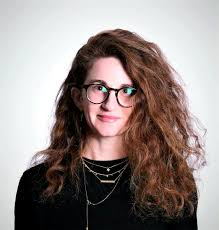
\includegraphics[
  width=0.82\linewidth,
  height=2.5cm,
  keepaspectratio
]{assets/havana.jpeg}

\vspace{0.35em}

\small
\textbf{Havana Rika}
\end{center}

% ---------------- right: references ----------------
\column{0.62\textwidth}

\textbf{This talk is based on four joint works:}

\vspace{0.6em}

\footnotesize

\begin{enumerate}
  \item \textit{Concept Learning for Algorithmic Reasoning: Insights from SAT-Solving GNNs}\\
  \textbf{Information Sciences}, 2026.

  \vspace{0.6em}

  \item \textit{From Black Box to Algorithmic Insight: Explainable AI in Graph Neural Networks for Graph Coloring}\\
  \textbf{AAAI 2025 NeurMAD Workshop }, 2025. 

  \vspace{0.6em}

  \item \textit{Learning to Rank: How GNNs Solve Max-Clique and Sparse PCA}\\
  \textbf{AAAI}, 2026.

  \vspace{0.6em}

  \item \textit{The Last Percent: Concept Emergence and the Jump from Approximation to Solving in Neural CSPs}\\
  \textbf{NeurIPS submission}, 2026. 
\end{enumerate}

\end{columns}

\end{frame}


% ══════════════════════════════════════════════════════════════════════════════
%  CHAPTER 1 — Crash Course: ML, GNNs, and the Promise
% ══════════════════════════════════════════════════════════════════════════════
\section{Chapter 0 — Motivation}


% ------------------------------------------------------------
% ── Slide 1 ──────────────────────────────────────────────────────────────

\begin{frame}{We have spent many years designing and analyzing algorithms }

\begin{center}
\resizebox{\textwidth}{!}{%
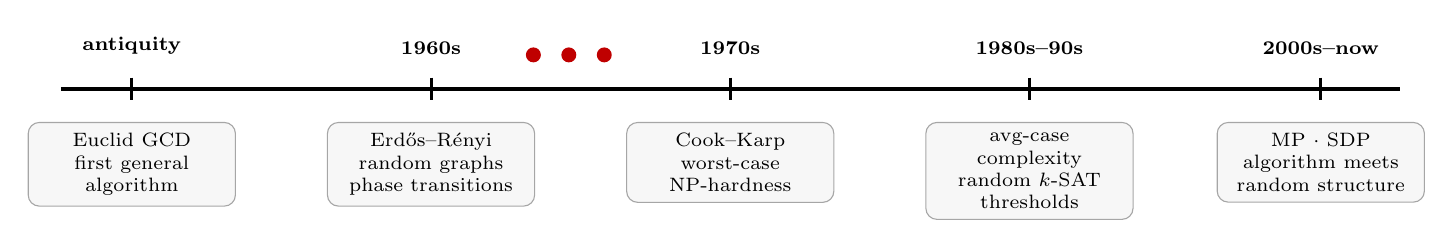
\begin{tikzpicture}[
    timeline/.style={line width=1.4pt},
    tick/.style={line width=1.1pt},
    yearlabel/.style={align=center, font=\scriptsize\bfseries},
    box/.style={
        rounded corners,
        draw=black!35,
        fill=black!3,
        inner sep=4pt,
        align=center,
        font=\scriptsize,
        text width=2.35cm,
        minimum height=0.95cm
    }
]
\draw[timeline] (0,0) -- (17.0,0);
\foreach \x in {6.0,6.45,6.9} {
    \fill[red!75!black] (\x,0.43) circle (0.095);
}
\foreach \x/\year/\txt in {
    0.9/{antiquity}/{Euclid GCD\\first general\\algorithm},
    4.7/{1960s}/{Erd\H{o}s--R\'enyi\\random graphs\\phase transitions},
    8.5/{1970s}/{Cook--Karp\\worst-case\\NP-hardness},
    12.3/{1980s--90s}/{avg-case complexity\\random $k$-SAT\\thresholds},
    16.0/{2000s--now}/{MP $\cdot$ SDP \\algorithm meets\\random structure}
}{
    \draw[tick] (\x,0.14) -- (\x,-0.14);
    \node[yearlabel, above=5pt] at (\x,0.14) {\year};
    \node[box, below=8pt] at (\x,-0.14) {\txt};
}
\end{tikzpicture}%
}
\end{center}

\vspace{1.5em}

\begin{block}{A unified framework}
\begin{itemize}
    \item \textbf{Design:} hand-craft an algorithm (for the worst/average case)
    \item \textbf{Structure:} identify what makes the problem tractable
    \item \textbf{Complexity:} bound time and space
    \item \textbf{Proof:} establish correctness and optimality
\end{itemize}
\end{block}

\end{frame}


% ------------------------------------------------------------
% ── Slide 2 ──────────────────────────────────────────────────────────────

\begin{frame}{I met Amin in 2006 in Humboldt}

\begin{center}

% Replace with the actual Dagstuhl photo filename.
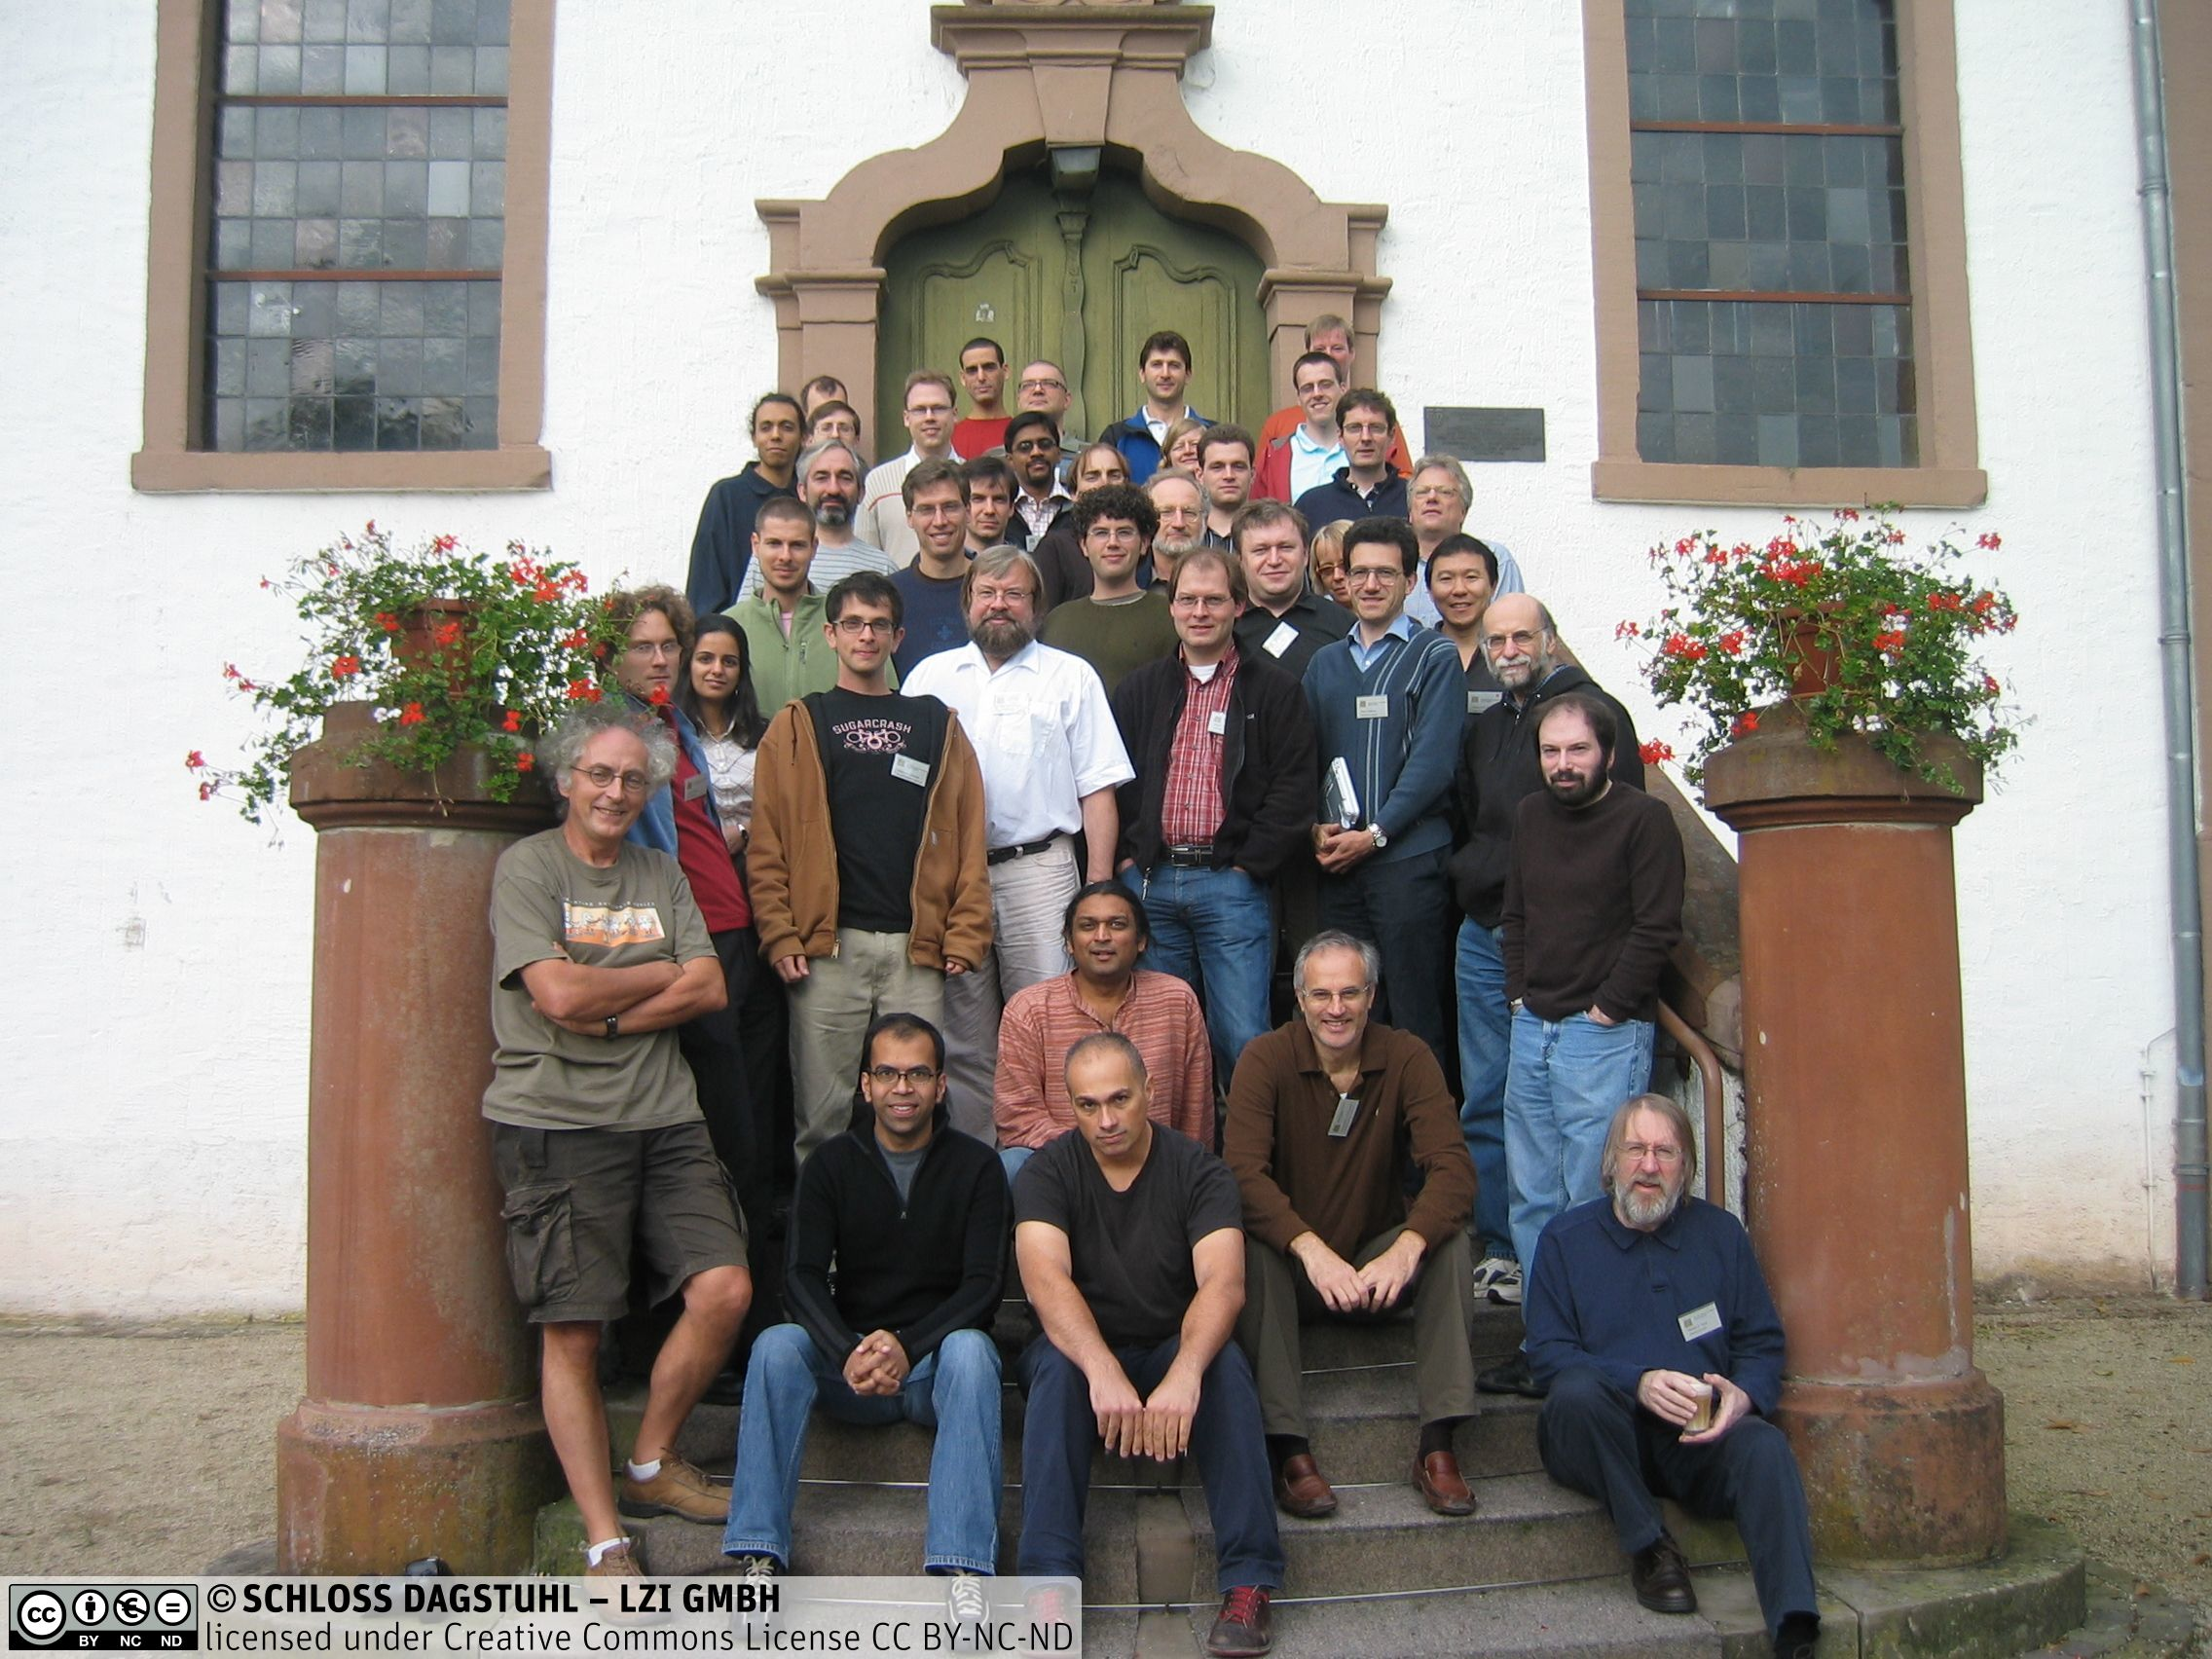
\includegraphics[width=0.72\textwidth,height=5.6cm,keepaspectratio]{assets/07391.01.l.jpg}

\vspace{0.8em}

\large
Dagstuhl 2007: \emph{Probabilistic Methods in the Design\\
and Analysis of Algorithms}

\end{center}

\end{frame}



% ------------------------------------------------------------
% ── Slide 3─────────────────────────────────────────────────

\begin{frame}{Then came the ML revolution}

\begin{columns}[T,onlytextwidth]

\column{0.54\textwidth}

\Large
A Wind of Change ??? \\

\vspace{0.50em}

\normalsize
Instead of hand-crafted rules, potential functions,
relaxations,  rounding schemes, (some) people began to ask:

\vspace{0.6em}

\begin{block}{Could learning replace manual design?}
\begin{itemize}
    \item Data-driven approach
    \item Learn everything end-to-end
    \item No mathematical guarantees -- Empirical evidence
    \item Generalization, Cross-Validation
\end{itemize}
\end{block}

\vspace{0.5em}



\column{0.42\textwidth}

\begin{center}
\vspace{0.1em}

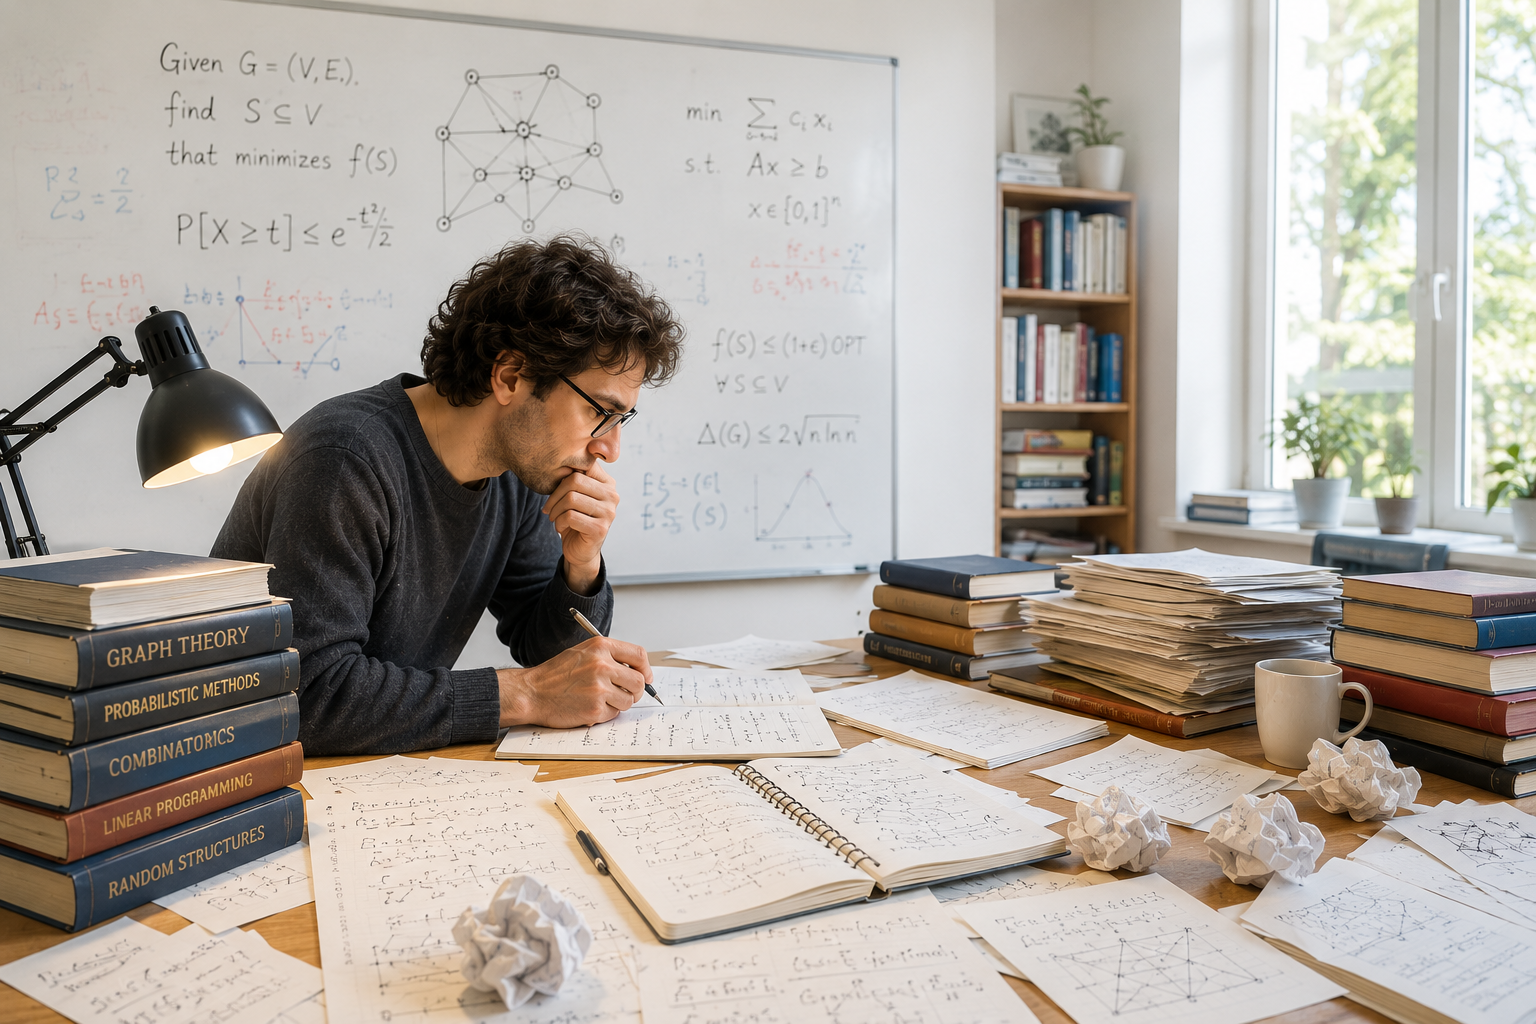
\includegraphics[width=0.92\linewidth,height=4.1cm,keepaspectratio]{assets/labor.png}
\end{center}

\end{columns}

\end{frame}


% ------------------------------------------------------------
% ── Slide 4─────────────────────────────────────────────────

% ------------------------------------------------------------
% ------------------------------------------------------------

\begin{frame}{Could DNNs learn something we don't know?}

\begin{columns}[c,onlytextwidth]

\column{0.56\textwidth}

\begin{block}{Could deep neural networks learn \emph{better algorithms}?}
\begin{itemize}
    \item Algorithms that work in parameter regimes where our current theory and hand-crafted methods struggle?
    \item Random SAT near the SAT/UNSAT threshold
    \item Can ML-based algorithms inform hand-crafted algorithm design and analysis?
    \item Or, the other way round?
\end{itemize}
\end{block}

\column{0.40\textwidth}

\begin{center}
\only<2->{
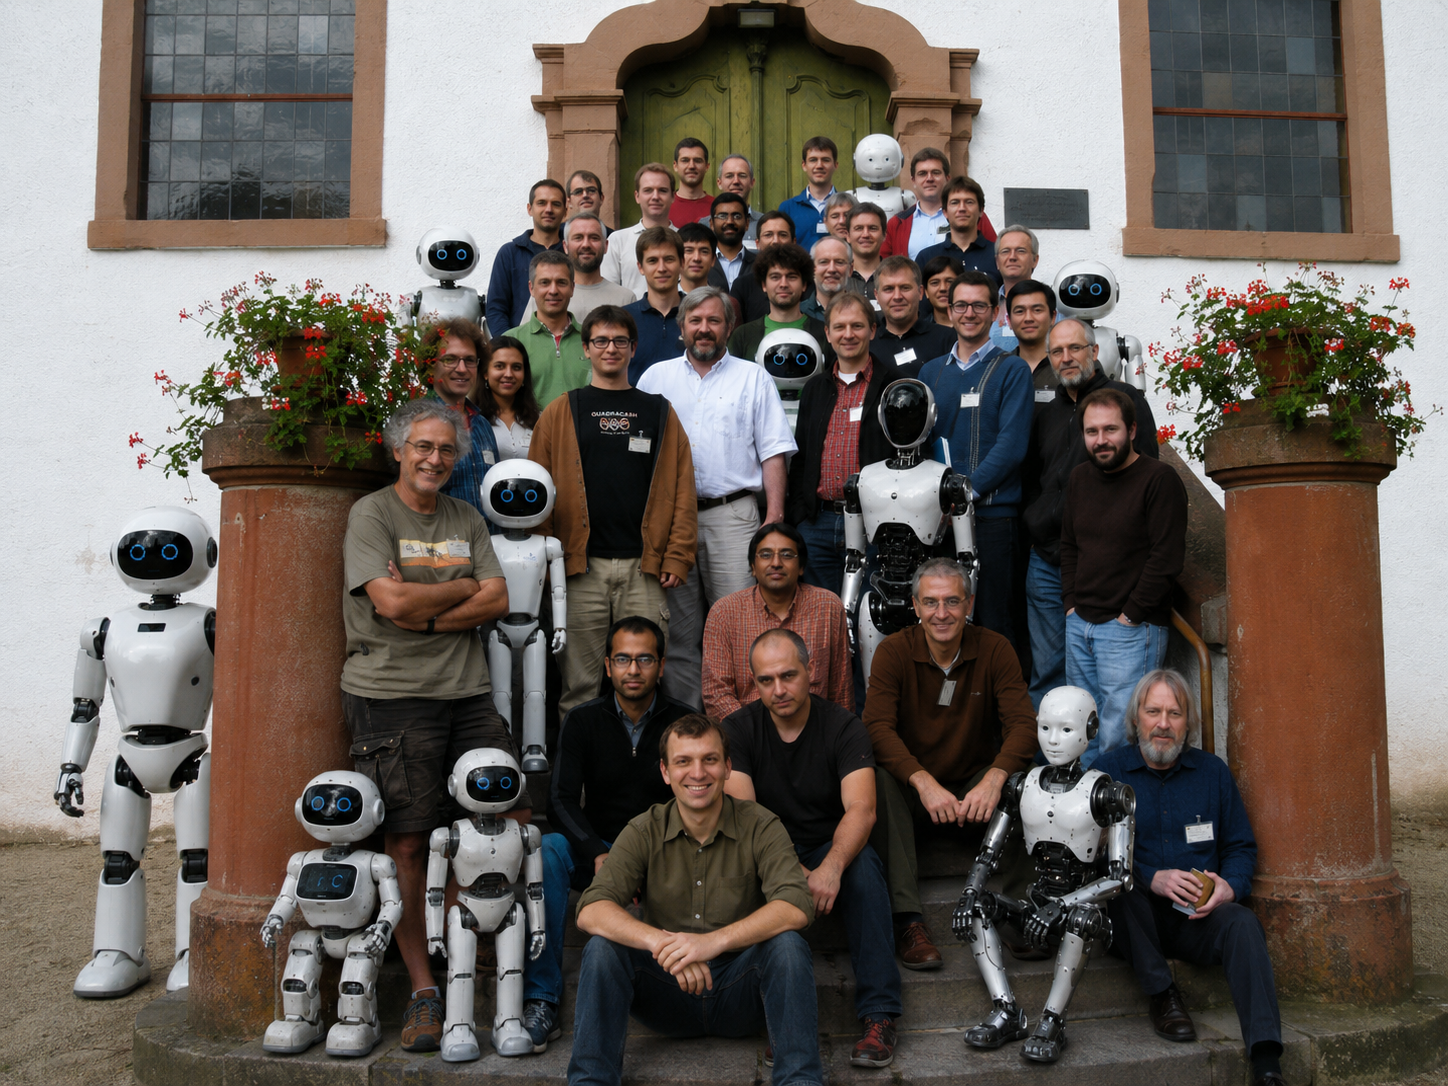
\includegraphics[width=\linewidth,height=5.4cm,keepaspectratio]{assets/Dagstul2037.png}

\vspace{0.35em}

\small
\textit{Dagstuhl 2037: The Design and Analysis of AI-generated Algorithms}
}
\end{center}

\end{columns}

\end{frame}

% ------------------------------------------------------------
% ── Slide 5─────────────────────────────────────────────────

% ------------------------------------------------------------
% ------------------------------------------------------------

\begin{frame}{The setting: combinatorial optimization on graphs}

\begin{columns}[c,onlytextwidth]

% ---------------- left: text ----------------
\column{0.74\textwidth}

\begin{itemize}
  \item \textbf{Input:} graph or a CNF formula
  \item \textbf{Goal (Search):} find an assignment to the variables satisfying all (or most) constraints
  \item \textbf{Goal (Decision):} decide if all constraints can be satisfied simultaneously
  \item \textbf{Challenge:} NP-complete in the worst case
\end{itemize}

\medskip

\onslide<2->{
\textbf{Problems in this talk:}
\begin{itemize}
  \item 3-\textbf{SAT}: assign TRUE/FALSE to variables
  \item \textbf{Coloring}: assign colors, no two adjacent vertices same
  \item \textcolor{gray!75}{{Max Clique}: find a large complete subgraph}
  \item \textcolor{gray!75}{{Sparse PCA}: recover a sparse signal from a covariance matrix}
\end{itemize}
}

% ---------------- right: factor graph ----------------
\column{0.24\textwidth}

\begin{center}
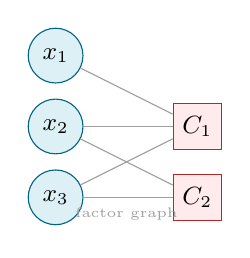
\begin{tikzpicture}[scale=0.72, every node/.style={font=\scriptsize}]
  % variable nodes
  \foreach \i/\lbl in {1/$x_1$, 2/$x_2$, 3/$x_3$} {
    \node[node, minimum size=5.8mm] (v\i) at (0, -1.25*\i+1.9) {\lbl};
  }

  % clause nodes
  \foreach \j/\lbl in {1/$C_1$, 2/$C_2$} {
    \node[clause, minimum size=5.8mm] (c\j) at (2.5, -1.25*\j+0.65) {\lbl};
  }

  % edges
  \draw[gray!75] (v1) -- (c1);
  \draw[gray!75] (v2) -- (c1);
  \draw[gray!75] (v2) -- (c2);
  \draw[gray!75] (v3) -- (c1);
  \draw[gray!75] (v3) -- (c2);

  \node[font=\tiny, color=gray!75] at (1.25, -2.15) {factor graph};
\end{tikzpicture}
\end{center}

\end{columns}



\end{frame}

% ------------------------------------------------------------
% ── Slide 6─────────────────────────────────────────────────

\begin{frame}{Supervised learning in 60 seconds: \NeuroSAT}

\begin{columns}[T,onlytextwidth]

\column{0.50\textwidth}

\textbf{General setup:}
\begin{itemize}
  \item Training data: \textit{(instance, label)} pairs
  \item Model: $f_\theta$: instance $\to$ prediction
  \item Loss: how wrong is $f_\theta$ vs.\ the label?
  \item Training: adjust $\theta$ to reduce loss (e.g., using SGD)
\end{itemize}

\bigskip

\onslide<2->{
\textbf{For \NeuroSAT\footnotemark:}
\begin{itemize}
  \item Instance: a SAT formula (incidence matrix)
  \item Label: \texttt{SAT} or \texttt{UNSAT} (one bit)
  \item Loss: cross-entropy on that single bit $y$,
\[
\mathcal{L}(y,\hat{p})
=
-\Big(y\log \hat{p} + (1-y)\log(1-\hat{p})\Big)
\]
\end{itemize}
}

\column{0.46\textwidth}

\begin{overlayarea}{\linewidth}{6.2cm}

\only<1-2>{
\begin{center}
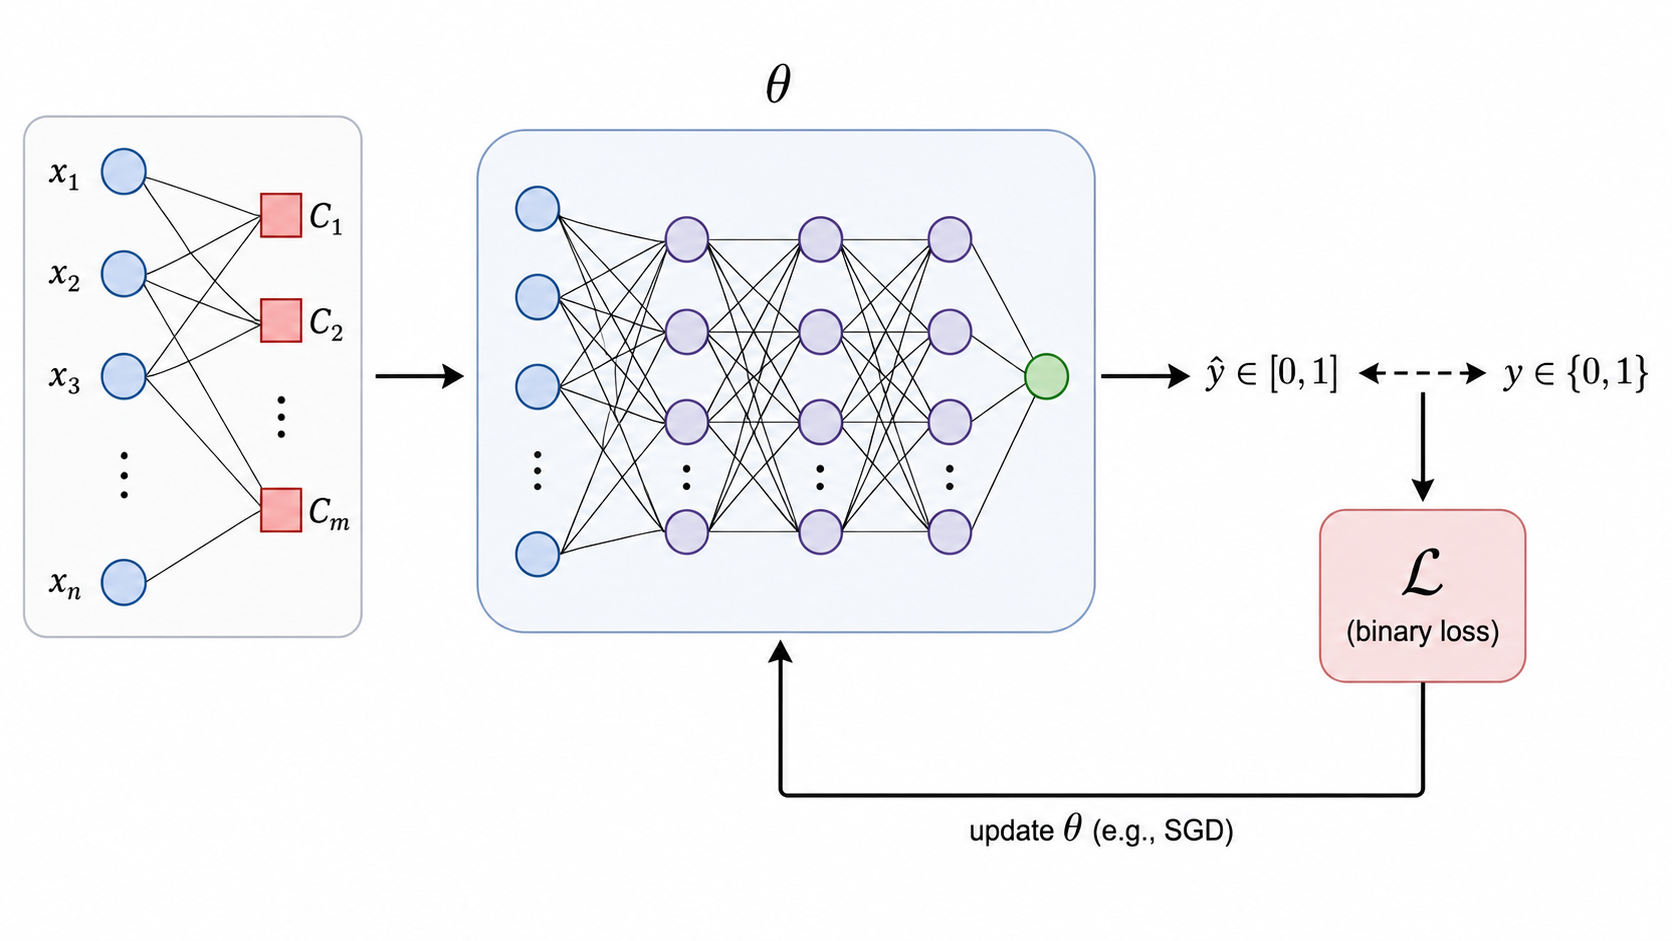
\includegraphics[width=\linewidth,height=6.2cm,keepaspectratio]{assets/train_pipe.png}
\end{center}
}

\only<3->{
\begin{block}{Key point}
\small
The loss does \emph{not} encode an algorithm:
no rules, no heuristics, no solver concepts.

\medskip
It only rewards the final SAT/UNSAT prediction.

\medskip
So if algorithmic concepts appear, they are hiding somewhere in the learned parameter space~$\theta$.
\end{block}
}

\end{overlayarea}

\end{columns}

\footnotetext{Selsam et al. (2019), \emph{Learning a SAT solver from single-bit supervision}, ICLR.}

\end{frame}

% ------------------------------------------------------------
% ── Slide 7─────────────────────────────────────────────────

% ------------------------------------------------------------
% ------------------------------------------------------------

\begin{frame}{Why would one hope for algorithmic concept learning?}

\begin{center}
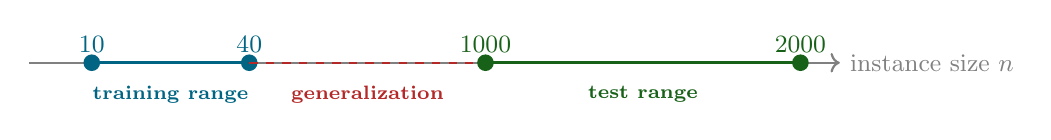
\begin{tikzpicture}[every node/.style={font=\small}]
  \draw[->, thick, gray] (-0.3,0) -- (10,0) node[right] {instance size $n$};
  % training range
  \draw[bgucolor, very thick] (0.5,0) -- (2.5,0);
  \fill[bgucolor] (0.5,0) circle(3pt) node[above] {$10$};
  \fill[bgucolor] (2.5,0) circle(3pt) node[above] {$40$};
  \node[bgucolor, font=\scriptsize] at (1.5, -0.4) {\textbf{training range}};
  % gap
  \draw[emphcolor, dashed, thick] (2.5,0) -- (5.5,0);
  \node[emphcolor, font=\scriptsize] at (4,-0.4) {\textbf{generalization}};
  % test range
  \draw[ForestGreen!70!black, very thick] (5.5,0) -- (9.5,0);
  \fill[ForestGreen!70!black] (5.5,0) circle(3pt) node[above] {1000};
  \fill[ForestGreen!70!black] (9.5,0) circle(3pt) node[above] {$2000$};
  \node[ForestGreen!70!black, font=\scriptsize] at (7.5,-0.4) {\textbf{test range}};
\end{tikzpicture}
\end{center}

\medskip
\begin{columns}[T]
\column{0.48\textwidth}
\textbf{Ordinary generalization:}\\same distribution, held-out examples
\column{0.48\textwidth}
\textbf{Size generalization:}\\test instances much larger than training
\end{columns}

\bigskip
\begin{alertblock}{}
\small
If the model generalizes across sizes:\\
$\Rightarrow$ it may have learned something \textbf{structural}, not instance-specific\\
$\Rightarrow$ that structural invariant is our object of study
\end{alertblock}

\end{frame}


\section{Chapter 1 — Preliminaries}
% ── Slide 7 ──────────────────────────────────────────────────────────────────
\begin{frame}{Four things to keep separate}
\small
\renewcommand{\arraystretch}{1.35}
\begin{tabular}{@{}p{3.0cm}p{5.0cm}p{3.2cm}@{}}
\toprule
\textbf{Component} & \textbf{What it is} & \textbf{Who decides} \\
\midrule
\textbf{Architecture} & how information flows (layers, message-passing graph) & researcher \\
\textbf{Parameters} $\theta$ & numerical values inside the model & \textcolor{red!70!black}{\textbf{learned from data}} \\
\textbf{Training objective} & what the model is rewarded for predicting & researcher \\
\textbf{Decoding strategy} & how output scores $\to$ discrete solution & researcher (could be post-training) \\
\bottomrule
\end{tabular}

\bigskip
\only<2->{
\begin{block}{When we say ``the model learned $X$''}
\small
$X$ lives in the \textbf{parameters} — not designed, not prescribed by the loss.\\
$X$ emerged from the interaction of architecture, objective, and data.
\end{block}
}

\end{frame}



\begin{frame}{Graph-structured problems need graph-structured models}

\begin{columns}[T,onlytextwidth]

\column{0.54\textwidth}
\begin{center}
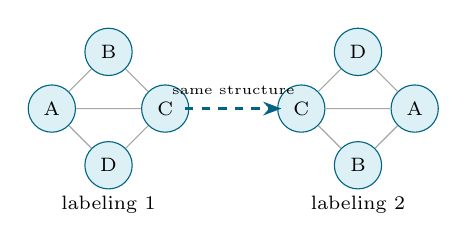
\begin{tikzpicture}[scale=0.72, every node/.style={font=\scriptsize}]

  % left graph
  \foreach \i/\x/\y in {A/0/1, B/1/2, C/2/1, D/1/0} {
    \node[circle, draw=bgucolor, fill=bgulight, minimum size=6mm] (\i) at (\x,\y) {\i};
  }
  \draw[gray!70] (A)--(B)--(C)--(D)--(A)--(C);
  \node at (1,-0.7) {labeling 1};

  % right graph, farther away
  \begin{scope}[xshift=4.4cm]
  \foreach \i/\x/\y in {C/0/1, D/1/2, A/2/1, B/1/0} {
    \node[circle, draw=bgucolor, fill=bgulight, minimum size=6mm] (\i r) at (\x,\y) {\i};
  }
  \draw[gray!70] (Cr)--(Dr)--(Ar)--(Br)--(Cr)--(Ar);
  \node at (1,-0.7) {labeling 2};
  \end{scope}

  % arrow with breathing room
  \draw[arrow, dashed] (2.35,1) -- (4.05,1);
  \node[font=\tiny, above] at (3.20,1.08) {same structure};

\end{tikzpicture}
\end{center}

\column{0.44\textwidth}
\hspace*{-0.35cm}
\begin{minipage}{\linewidth}

\textbf{Challenge:}\\
same graph, different node labels $\to$ same structure

\medskip

Standard NN: \alert{fails} \\
{\small no permutation invariance}

\medskip

\onslide<2->{
GNN: \textcolor{ForestGreen!70!black}{\textbf{operates on structure}} $\checkmark$

\medskip

\textbf{Also:}
\begin{itemize}\small
  \item GNNs support variable-size graphs naturally
  \item GNNs are message passing algorithms (fit local constraint structure)
\end{itemize}
}

\end{minipage}

\end{columns}

\note{Combinatorial problems on graphs are permutation-invariant. GNNs are built
for this. They also scale linearly with the number of edges, making them usable on large sparse
instances.}

\end{frame}

% ── Slide 9 ──────────────────────────────────────────────────────────────────
\begin{frame}{What is a GNN?}
\begin{columns}[T]
\column{0.48\textwidth}
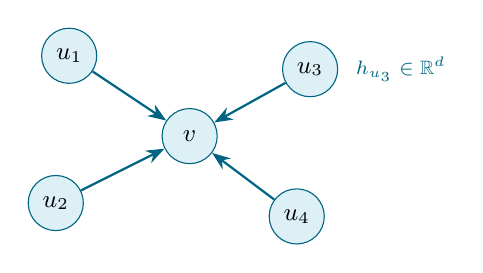
\begin{tikzpicture}[scale=0.85, every node/.style={font=\small}]
  \node[node] (v) at (2,2) {$v$};
  \node[node] (u1) at (0.2,3.2) {$u_1$};
  \node[node] (u2) at (0,1.0) {$u_2$};
  \node[node] (u3) at (3.8,3.0) {$u_3$};
  \node[node] (u4) at (3.6,0.8) {$u_4$};
  \draw[arrow] (u1) -- (v);
  \draw[arrow] (u2) -- (v);
  \draw[arrow] (u3) -- (v);
  \draw[arrow] (u4) -- (v);
  \node[font=\scriptsize, bgucolor, right=0.1cm of u3] {$h_{u_3}\in\mathbb{R}^d$};
\end{tikzpicture}

\column{0.48\textwidth}
Each vertex $v$ has a state $h_v \in \mathbb{R}^d$

\medskip
\textbf{Each round $t$:}
\[
  m_v \;=\; \mathrm{AGG}\!\bigl(\{h_u : u\in\mathcal{N}(v)\}\bigr)
\]
\[
  h_v \;\leftarrow\; \mathrm{UPDATE}(h_v,\, m_v)
\]

\medskip
After $T$ rounds: \textbf{predict} from $\{h_v\}$

\medskip\small
\texttt{AGG} and \texttt{UPDATE} are \textbf{learned} (e.g., MLP/RNN).\\
After $T$ rounds: $v$ has seen its $T$-hop neighborhood.
\end{columns}
\note{Think of it as a distributed algorithm where each node keeps a memory
vector and exchanges messages with its neighbors. The only difference from a designed algorithm
is that AGG and UPDATE are learned. What they learn to compute — that's our question.}
\end{frame}


\begin{frame}{NeuroSAT: One message passing step}

\vspace{-0.4em}

\begin{center}
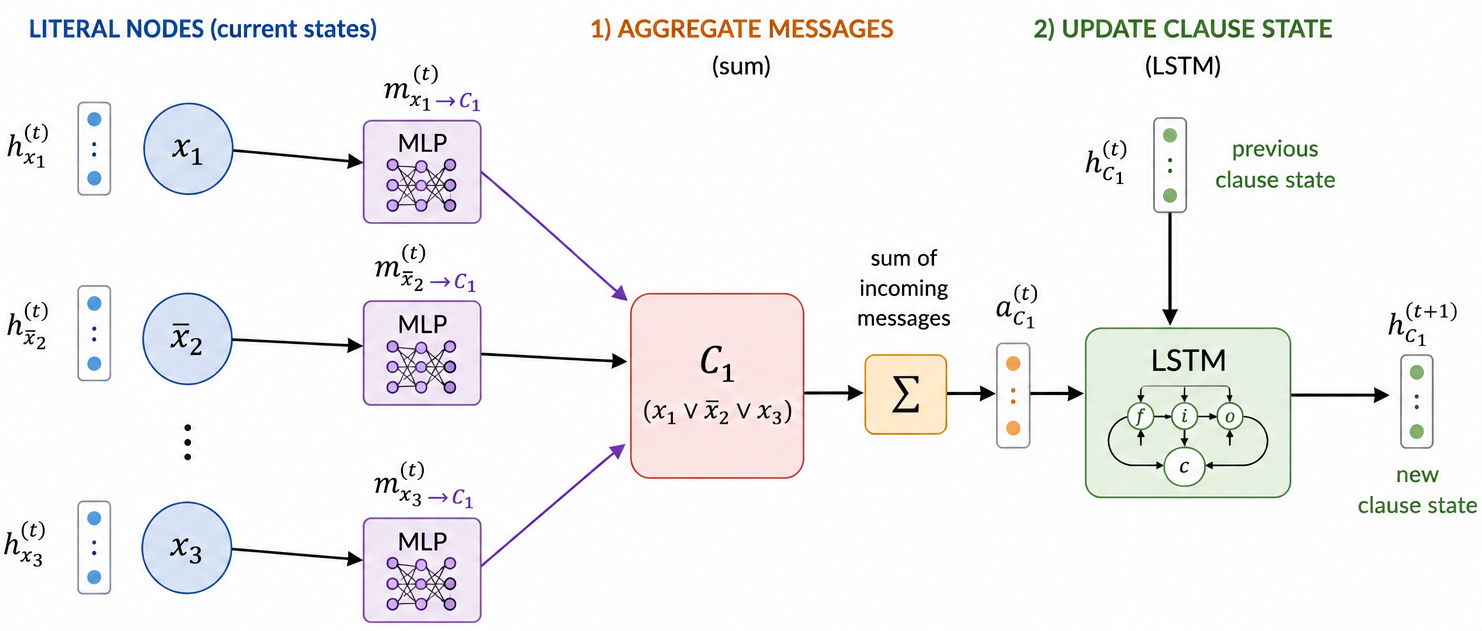
\includegraphics[
  width=0.98\linewidth,
  height=0.76\textheight,
  keepaspectratio
]{assets/one-message-passing.png}
\end{center}

\end{frame}


\begin{frame}{\NeuroSAT: Voting on satisfiability}

\vspace{-0.4em}

\begin{center}
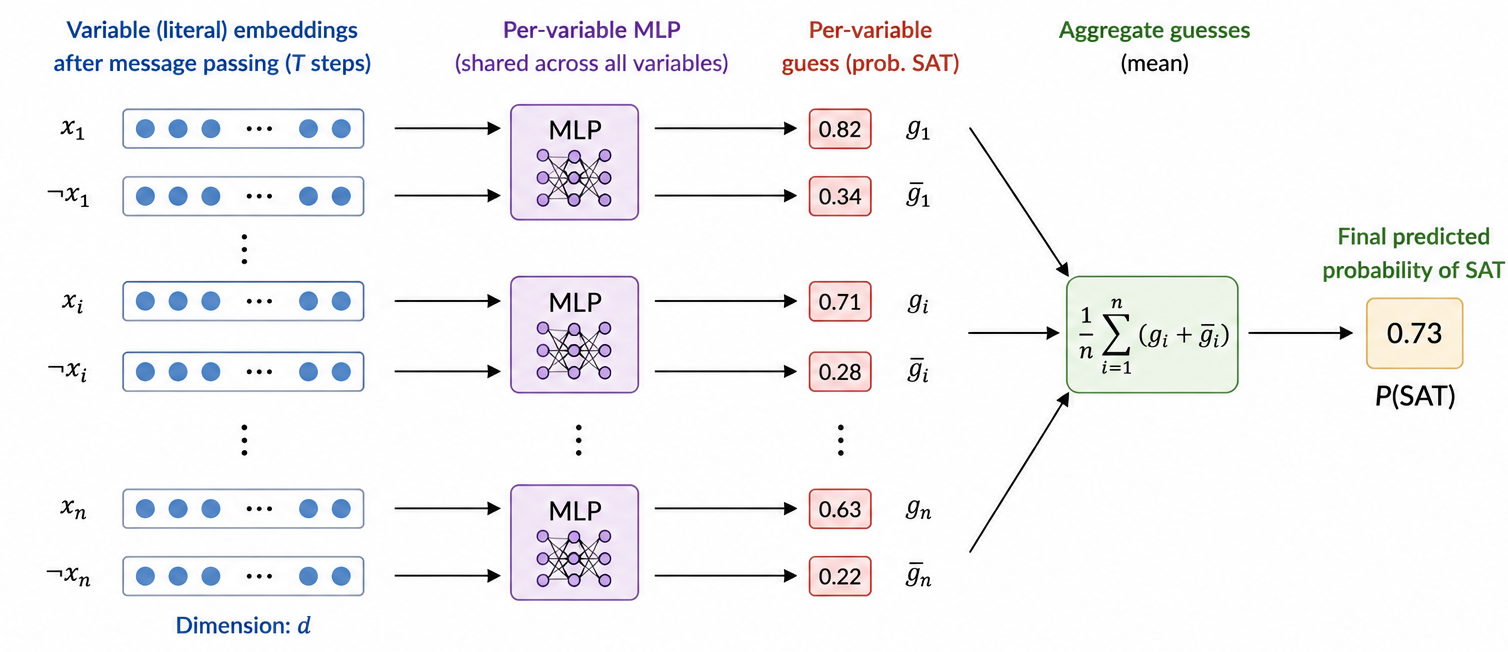
\includegraphics[
  width=0.98\linewidth,
  height=0.76\textheight,
  keepaspectratio
]{assets/vote.png}
\end{center}

\end{frame}
% ── Slide 11 ─────────────────────────────────────────────────────────────────
\begin{frame}{Belief propagation: the classical template}

\begin{center}
\renewcommand{\arraystretch}{1.4}
\begin{tabular}{@{}p{3.5cm}p{3.8cm}p{3.8cm}@{}}
\toprule
 & \textbf{BP} & \textbf{GNN} \\
\midrule
\textbf{Message} & scalar / probability & vector $\in \mathbb{R}^d$ \\
\textbf{Update rule} & analytically derived & learned (MLP/LSTM) \\
\textbf{Objective} & probabilistic model & task loss (SAT/UNSAT) \\
\textbf{Convergence} & proven on trees & empirical \\
\textcolor{red!75!black}{\textbf{Interpretability}} & high & \textcolor{red!75!black}{\textbf{our question}} \\
\bottomrule
\end{tabular}
\end{center}


\end{frame}

\section{Chapter 2 - Results}

\begin{frame}{From XAI to concept learning}

\small
\textbf{Explainable AI (XAI)} asks: how did the model arrive at this decision?

\medskip
\textbf{Concept learning}: we ask whether the model has learned
human-interpretable concepts.

\medskip

\begin{columns}[T,onlytextwidth]
\column{0.58\textwidth}
\centering
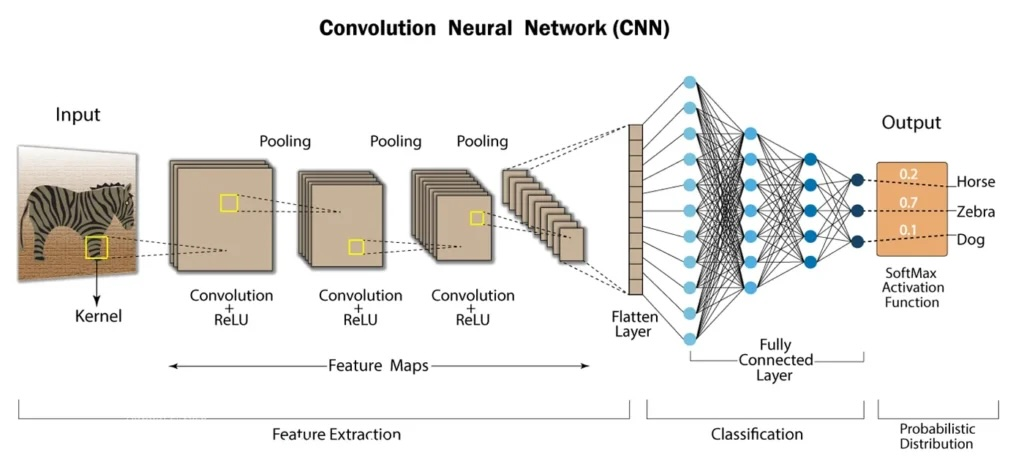
\includegraphics[width=\linewidth]{assets/cnn.jpeg}
\medskip

\column{0.38\textwidth}
\centering
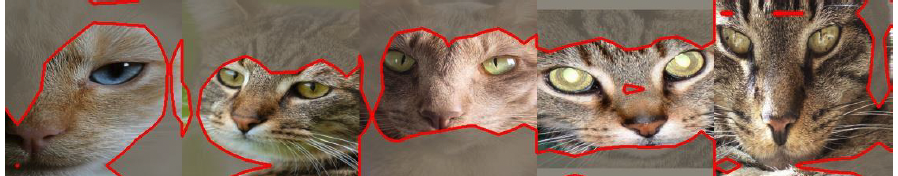
\includegraphics[width=\linewidth]{assets/concept.png}
\medskip

\small A possible learned concept: \textbf{eyes}.
\end{columns}

\medskip

\begin{block}{How can we find such concepts?}
\small
Perturb part of the input and check
whether the classification deteriorates.  
If it does, trace the affected activation back to the image region it corresponds to.
\end{block}

\end{frame}

% ── Slide 18 

\begin{frame}{Why algorithmic concepts are harder}

\small
In vision, a concept can often be tied to a visible region: eyes, wheels, wings.

\medskip
For algorithms, the ``concept'' is harder to pin down.

\begin{itemize}
    \item It depends on the instance and on the algorithm's current state
    \item So it is dynamic: it evolves over time
    \item It is not obvious where to look: NN parameters, hidden states?
\end{itemize}

\medskip
\onslide<2->{
\begin{block}{Philosophical problem}
\small
\begin{itemize}
    \item In vision, we do not need to know the concept in advance---we can search over image regions
    \item For algorithms, it is unclear how to search for a concept we do not already know
\end{itemize}
\end{block}
}

\end{frame}

% ------------------------------------------------------------

\begin{frame}{Meta-concept: Confidence}

\onslide<1->{
\begin{block}{General idea}
Given an instance \(I\), a current assignment \(\sigma\), and a vertex \(v\),  
it's useful to have a score that measures how confident we are that \(\sigma(v)\) is ``correct.''
\end{block}
}

\vspace{0.35em}

\onslide<2->{
\textbf{Useful means:}
}

\begin{itemize}
    \item<2-> \textbf{Computable:} it should be easy to compute from the information we have:
    \[
    \operatorname{conf}_{I,\sigma}(v) = g(I,\sigma,v).
    \]

    \item<3-> \textbf{Algorithmically actionable:} it guides the algorithm:
    \[
    \text{high } \operatorname{conf}_{I,\sigma}(v)
    \quad \Longrightarrow \quad
    \text{do not flip } \sigma(v).
    \]
\end{itemize}

\vspace{0.35em}

\onslide<4->{
\smallskip
\textbf{Correct} means: \(\sigma(v)\) agrees with \(v\)'s value in some satisfying solution.
}

\end{frame}

% ------------------------------------------------------------
\begin{frame}{Confidence in graph 3-coloring}

\begin{columns}[c,onlytextwidth]

% ---------------- left: toy graph ----------------
\column{0.48\textwidth}

\begin{center}
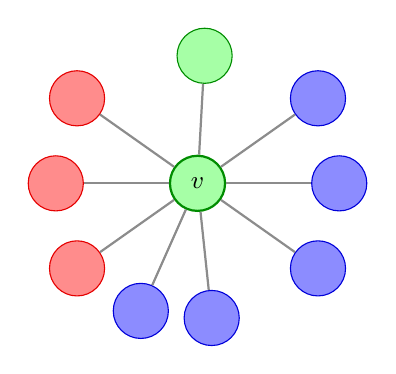
\begin{tikzpicture}[
    scale=0.9,
    every node/.style={font=\small},
    vgreen/.style={circle, draw=green!55!black, fill=green!35, minimum size=7mm},
    vblue/.style ={circle, draw=blue!85!black,  fill=blue!45,  minimum size=7mm},
    vred/.style  ={circle, draw=red!90!black,   fill=red!45,   minimum size=7mm},
    edge/.style={line width=0.8pt, black!45}
]

% center vertex
\node[vgreen, thick] (v) at (0,0) {$v$};

% red neighbors
\node[vred] (r1) at (-1.7,1.2) {};
\node[vred] (r2) at (-2.0,0.0) {};
\node[vred] (r3) at (-1.7,-1.2) {};

% blue neighbors
\node[vblue] (b1) at (1.7,1.2) {};
\node[vblue] (b2) at (2.0,0.0) {};
\node[vblue] (b3) at (1.7,-1.2) {};
\node[vblue] (b4) at (0.2,-1.9) {};
\node[vblue] (b5) at (-0.8,-1.8) {};

% one green neighbor
\node[vgreen] (g1) at (0.1,1.8) {};

% edges from v
\foreach \u in {r1,r2,r3,b1,b2,b3,b4,b5,g1} {
    \draw[edge] (v) -- (\u);
}

\end{tikzpicture}
\end{center}

% ---------------- right: definition ----------------
\column{0.49\textwidth}

\textbf{Current coloring:} \(\sigma(v)=\textcolor{green!45!black}{\text{green}}\).

\medskip

For a vertex \(v\), count its neighbors in each \emph{other} color class:

\[
d_{\textcolor{red!90!black}{R}}(v)
=
|\{u\in N(v):\sigma(u)=\textcolor{red!90!black}{R}\}|,
\]

\[
d_{\textcolor{blue!85!black}{B}}(v)
=
|\{u\in N(v):\sigma(u)=\textcolor{blue!85!black}{B}\}|.
\]

\medskip

\[
\operatorname{conf}_{\sigma}(v)
=
\min\left\{
d_{\textcolor{red!90!black}{R}}(v),
d_{\textcolor{blue!85!black}{B}}(v)
\right\}.
\]

\medskip

Many red and blue neighbors \(\Rightarrow\) changing \(v\)'s color is costly.

\end{columns}

\medskip


\vfill

{\small
``A spectral technique for coloring random 3-colorable graphs", 
Alon and Kahale, STOC 1994.
}

\end{frame}

% ------------------------------------------------------------
\begin{frame}{Support as confidence in SAT}

\begin{columns}[T,onlytextwidth]

% ============================================================
% Left: clause flip illustration + definition
% ============================================================
\column{0.73\textwidth}

\begin{center}
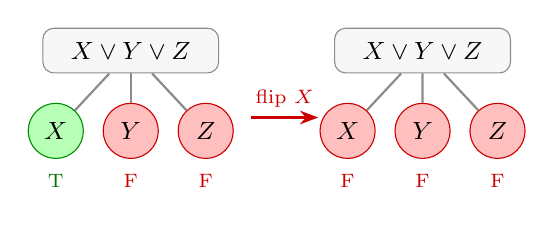
\begin{tikzpicture}[
    scale=0.68,
    every node/.style={font=\small},
    litT/.style={circle, draw=green!55!black, fill=green!28, minimum size=7mm},
    litF/.style={circle, draw=red!80!black, fill=red!25, minimum size=7mm},
    clausebox/.style={rounded corners, draw=black!45, fill=black!3, inner sep=5pt},
    arrow/.style={->, thick, >=Stealth},
    edge/.style={line width=0.8pt, black!45}
]

% ---------------- before flip ----------------
\node[clausebox] (clause) at (0,1.35) {
\(\;\; X \vee Y \vee Z \;\;\)
};

\node[litT] (x) at (-1.4,-0.15) {\(X\)};
\node[litF] (y) at (0,-0.15) {\(Y\)};
\node[litF] (z) at (1.4,-0.15) {\(Z\)};

\node[below=2pt of x, font=\scriptsize, green!45!black] {T};
\node[below=2pt of y, font=\scriptsize, red!80!black] {F};
\node[below=2pt of z, font=\scriptsize, red!80!black] {F};

\draw[edge] (x) -- (clause);
\draw[edge] (y) -- (clause);
\draw[edge] (z) -- (clause);

% ---------------- arrow ----------------
\draw[arrow, red!80!black] (2.25,0.1) -- (3.50,0.1)
node[midway, above, font=\scriptsize] {flip \(X\)};

% ---------------- after flip ----------------
\node[clausebox] (clause2) at (5.45,1.35) {
\(\;\; X \vee Y \vee Z \;\;\)
};

\node[litF] (x2) at (4.05,-0.15) {\(X\)};
\node[litF] (y2) at (5.45,-0.15) {\(Y\)};
\node[litF] (z2) at (6.85,-0.15) {\(Z\)};

\node[below=2pt of x2, font=\scriptsize, red!80!black] {F};
\node[below=2pt of y2, font=\scriptsize, red!80!black] {F};
\node[below=2pt of z2, font=\scriptsize, red!80!black] {F};

\draw[edge] (x2) -- (clause2);
\draw[edge] (y2) -- (clause2);
\draw[edge] (z2) -- (clause2);

\end{tikzpicture}
\end{center}

\vspace{0.35em}

{\small
A variable \(x\) \textbf{supports} a clause \(C\) if \(C\) is satisfied and
\(x\) is the \emph{only} literal satisfying it.
}

\vspace{-0.15em}

\[
\operatorname{supp}_{\sigma}(x)
=
\left|
\{C:\; x \text{ is the only satisfying literal of } C\}
\right|.
\]

\vspace{0.2em}

{\small\textcolor{blue!70!black}{
High support \(\Rightarrow\) flipping \(x\) breaks many clauses.
}}
% 
% Right: compact support graph
% ============================================================
\column{0.24\textwidth}

\vspace{0.25em}

\begin{center}
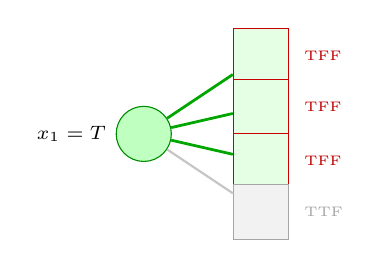
\begin{tikzpicture}[
    scale=0.62,
    every node/.style={font=\scriptsize},
    litT/.style={circle, draw=green!55!black, fill=green!25, minimum size=7mm},
    clauseTFF/.style={rectangle, draw=red!80!black, fill=green!10, minimum size=7mm},
    clauseOther/.style={rectangle, draw=gray!70, fill=gray!10, minimum size=7mm},
    edgeT/.style={line width=1.0pt, green!65!black},
    edgeOther/.style={line width=0.8pt, gray!45}
]

\node[litT, label=left:{\scriptsize \(x_1=T\)}] (x) at (0,0) {};

\node[clauseTFF] (c1) at (2.4,1.6) {};
\node[clauseTFF] (c2) at (2.4,0.55) {};
\node[clauseTFF] (c3) at (2.4,-0.55) {};
\node[clauseOther] (c4) at (2.4,-1.6) {};

\draw[edgeT] (x) -- (c1);
\draw[edgeT] (x) -- (c2);
\draw[edgeT] (x) -- (c3);
\draw[edgeOther] (x) -- (c4);

\node[right=2pt of c1, font=\tiny, red!75!black] {TFF};
\node[right=2pt of c2, font=\tiny, red!75!black] {TFF};
\node[right=2pt of c3, font=\tiny, red!75!black] {TFF};
\node[right=2pt of c4, font=\tiny, gray!70] {TTF};

\end{tikzpicture}
\end{center}

\end{columns}

\medskip

{\scriptsize
Support appeared in various random SAT papers:
\emph{``A spectral technique for random satisfiable 3CNF formulas''}, Flaxman, 2003;
\emph{``Why almost all \(k\)-CNF formulas are easy''}, Coja-Oghlan, Krivelevich, and Vilenchik, 2007;
\emph{``Algorithmic Barriers from Phase Transitions''}, Achlioptas and Coja-Oghlan, 2008.
}

\end{frame}

% ------------------------------------------------------------
\begin{frame}{Where we are so far}

\vspace{0.6em}

\begin{itemize}
    \item[\textcolor{green!55!black}{\Large\(\checkmark\)}]
    \normalsize \textbf{Graph Neural Networks:}
    learned message-passing algorithms on graphs / factor graphs

    \vspace{0.4em}

    \item[\textcolor{green!55!black}{\Large\(\checkmark\)}]
    \normalsize \textbf{Algorithmic concepts:}
    computable, actionable signals that guide a solver

    \vspace{0.4em}

    \item[\textcolor{green!55!black}{\Large\(\checkmark\)}]
    \normalsize \textbf{Coloring confidence:}
    minimum degree into the other color classes

    \vspace{0.4em}

    \item[\textcolor{green!55!black}{\Large\(\checkmark\)}]
    \normalsize \textbf{SAT confidence:}
    support — clauses where a variable is the only satisfying literal
\end{itemize}

\vspace{0.8em}

\onslide<2->{
\begin{center}
\begin{minipage}{0.60\textwidth}
\begin{block}{Now the question}
\centering
Does the GNN learn these concepts?\\
And if so, how does it use them?
\end{block}
\end{minipage}
\end{center}
}

\end{frame}

% ------------------------------------------------------------
\begin{frame}{What we will see}

\centering
\renewcommand{\arraystretch}{1.55}
\small

\begin{tabular}{@{}p{2.1cm}p{2.8cm}c p{5.0cm}@{}}
\toprule
\textbf{Model} & \textbf{Architecture} & \textbf{Concept?} & \textbf{Outcome} \\
\midrule

\textbf{\NeuroSAT}
&
Supervised
&
\textcolor{green!55!black}{\Large\(\checkmark\)}
&
Solves random SAT ``well"
\\

\midrule

\textbf{\GCP}
&
Supervised
&
\textcolor{orange}{\Large\(\boldsymbol{?}\)}
&
Solves \(\sim 5\%\) of 3-colorable graphs; succeeds where confidence is learned
\\

\midrule

\textbf{\OptGNN}
&
Unsupervised, SDP-inspired
&
\textcolor{red!75!black}{\Large\(\times\)}
&
Approximates well \((\sim 99\%)\), but does not  solve SAT
\\

\bottomrule
\end{tabular}

\medskip

\onslide<2->{
\vspace{0.7em}
\begin{center}
\begin{minipage}{0.77\textwidth}
\begin{block}{Conjecture}
\centering
Exact solving (for random CSPs) happens when the GNN is learning an actionable confidence concept
\end{block}
\end{minipage}
\end{center}
}

\end{frame}


% ------------------------------------------------------------
\begin{frame}{Why should we care what concept the GNN learned?}

\small

\begin{itemize}
    \item<1-> \textbf{Comparing GNNs:}
    A new paper claims a ``superior GNN'' with a \(+\varepsilon\) improvement.\\
    Is it learning a new algorithmic idea, or just optimizing the same concept better?

    \vspace{0.25em}

    \item<2-> \textbf{Simplification:}
    Identify the minimal architecture that still solves the task.\\
    Can we replace an LSTM with a simpler RNN?

    \vspace{0.25em}

    \item<3-> \textbf{Toward rigorous analysis:}
    Once the GNN is simplified, we may have a chance to prove something about it.

    \vspace{0.25em}

    \item<4-> \textbf{Explaining out-of-distribution failure:}
    If the model fails on, say, non-random instances, concept analysis can tell us why.

    \vspace{0.25em}

    \item<5-> \textbf{Fixing architectures that fail:}
    If a model approximates but does not solve, concept analysis can steer augmentations.\\

    \vspace{0.25em}

    \item<6-> \textbf{Returning insight to algorithms:}
    Can a GNN solve something that no classical heuristic has managed to? Did it learn something new?
\end{itemize}

\end{frame}


\section{Chapter 3 - NeuroSAT}

% ------------------------------------------------------------
\begin{frame}{Case Study: {\rmfamily\textsc{NeuroSAT}} }

\begin{center}
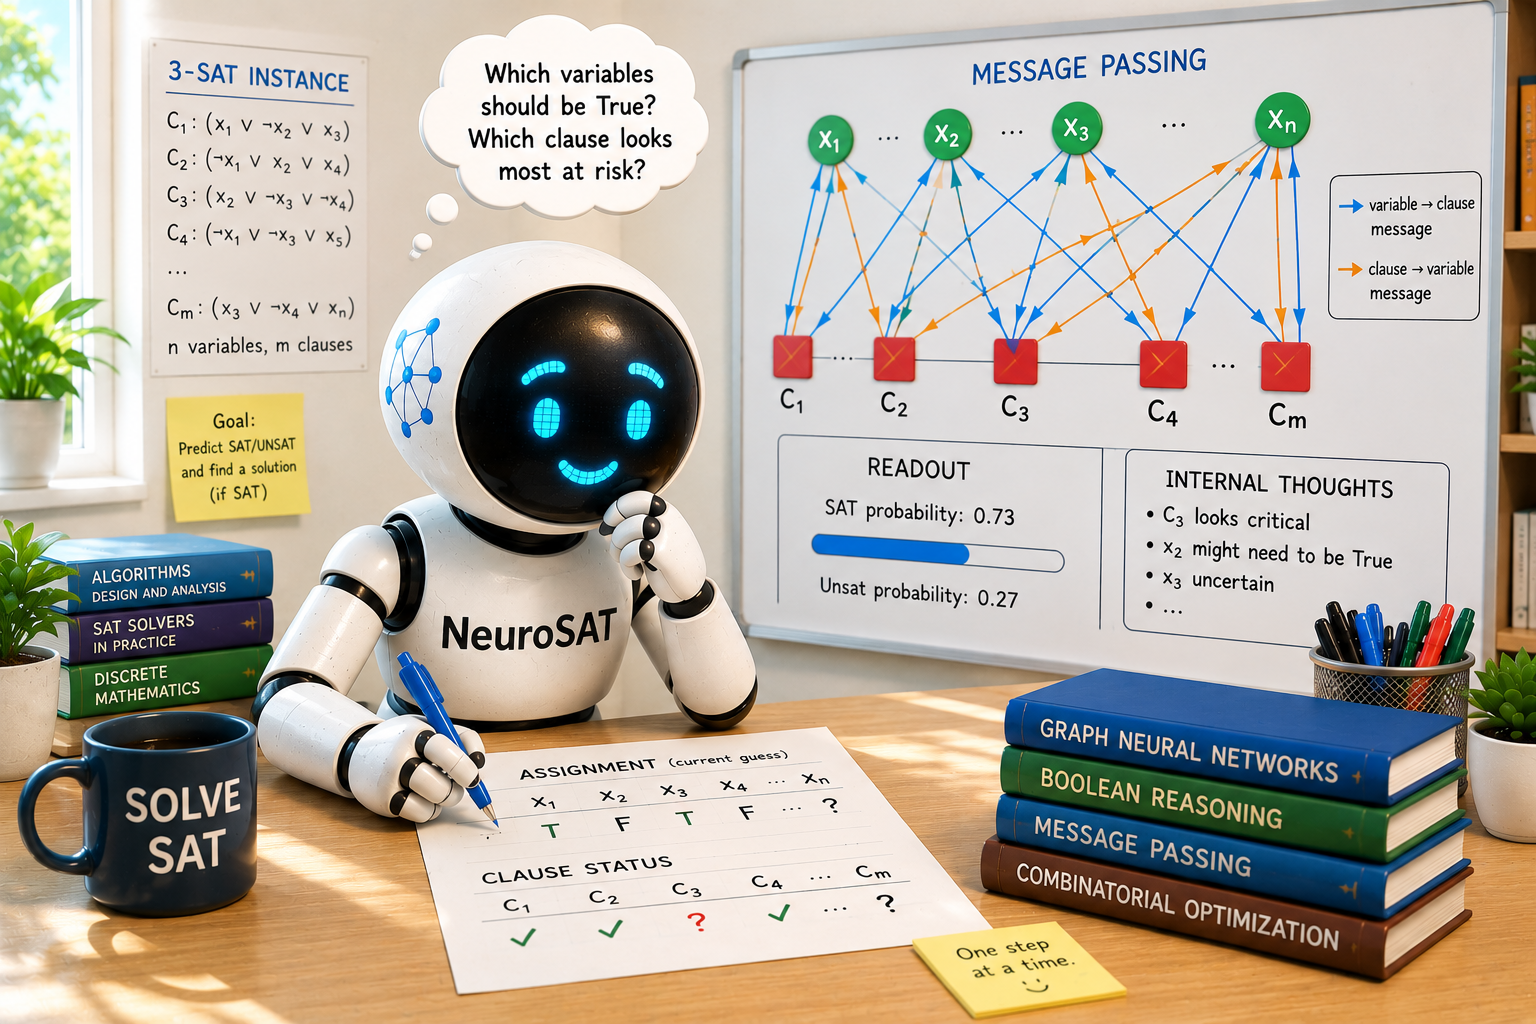
\includegraphics[
  width=\linewidth,
  height=0.82\textheight,
  keepaspectratio
]{assets/neurosat-ai.png}
\end{center}

\end{frame}

% ------------------------------------------------------------
\begin{frame}{Training Set for NeuroSAT}

\small

\begin{center}
\begin{minipage}{0.88\textwidth}
\hrule
\vspace{0.45em}

\textbf{Generate 1M SAT/UNSAT training pair}

\vspace{0.35em}

\begin{tabular}{@{}ll@{}}
1. & Choose \(n \in \{10,\ldots,40\}\). \\[0.2em]
2. & Start with an empty formula \(F\). \\[0.2em]
3. & \textbf{while} \(F\) is \texttt{SAT} \textbf{do} \\[0.2em]
   & \quad Sample a random 3-SAT clause \(C\). \\[0.2em]
   & \quad Set \(F' \gets F \wedge C\). \\[0.2em]
   & \quad Check \(F'\) with an exact SAT solver. \\[0.2em]
   & \quad \textbf{if} \(F'\) is \texttt{SAT} \textbf{then} \\[0.2em]
   & \quad\quad \(F \gets F'\). \\[0.2em]
   & \quad \textbf{else} \\[0.2em]
   & \quad\quad \textbf{return} \((F,\texttt{SAT})\) and \((F',\texttt{UNSAT})\). \\[0.2em]
   & \quad \textbf{end if} \\[0.2em]
4. & \textbf{end while}
\end{tabular}

\vspace{0.45em}
\hrule
\end{minipage}
\end{center}


\end{frame}

% ------------------------------------------------------------
\begin{frame}{NeuroSAT performance}

\begin{columns}[c,onlytextwidth]

\column{0.49\textwidth}
\begin{center}
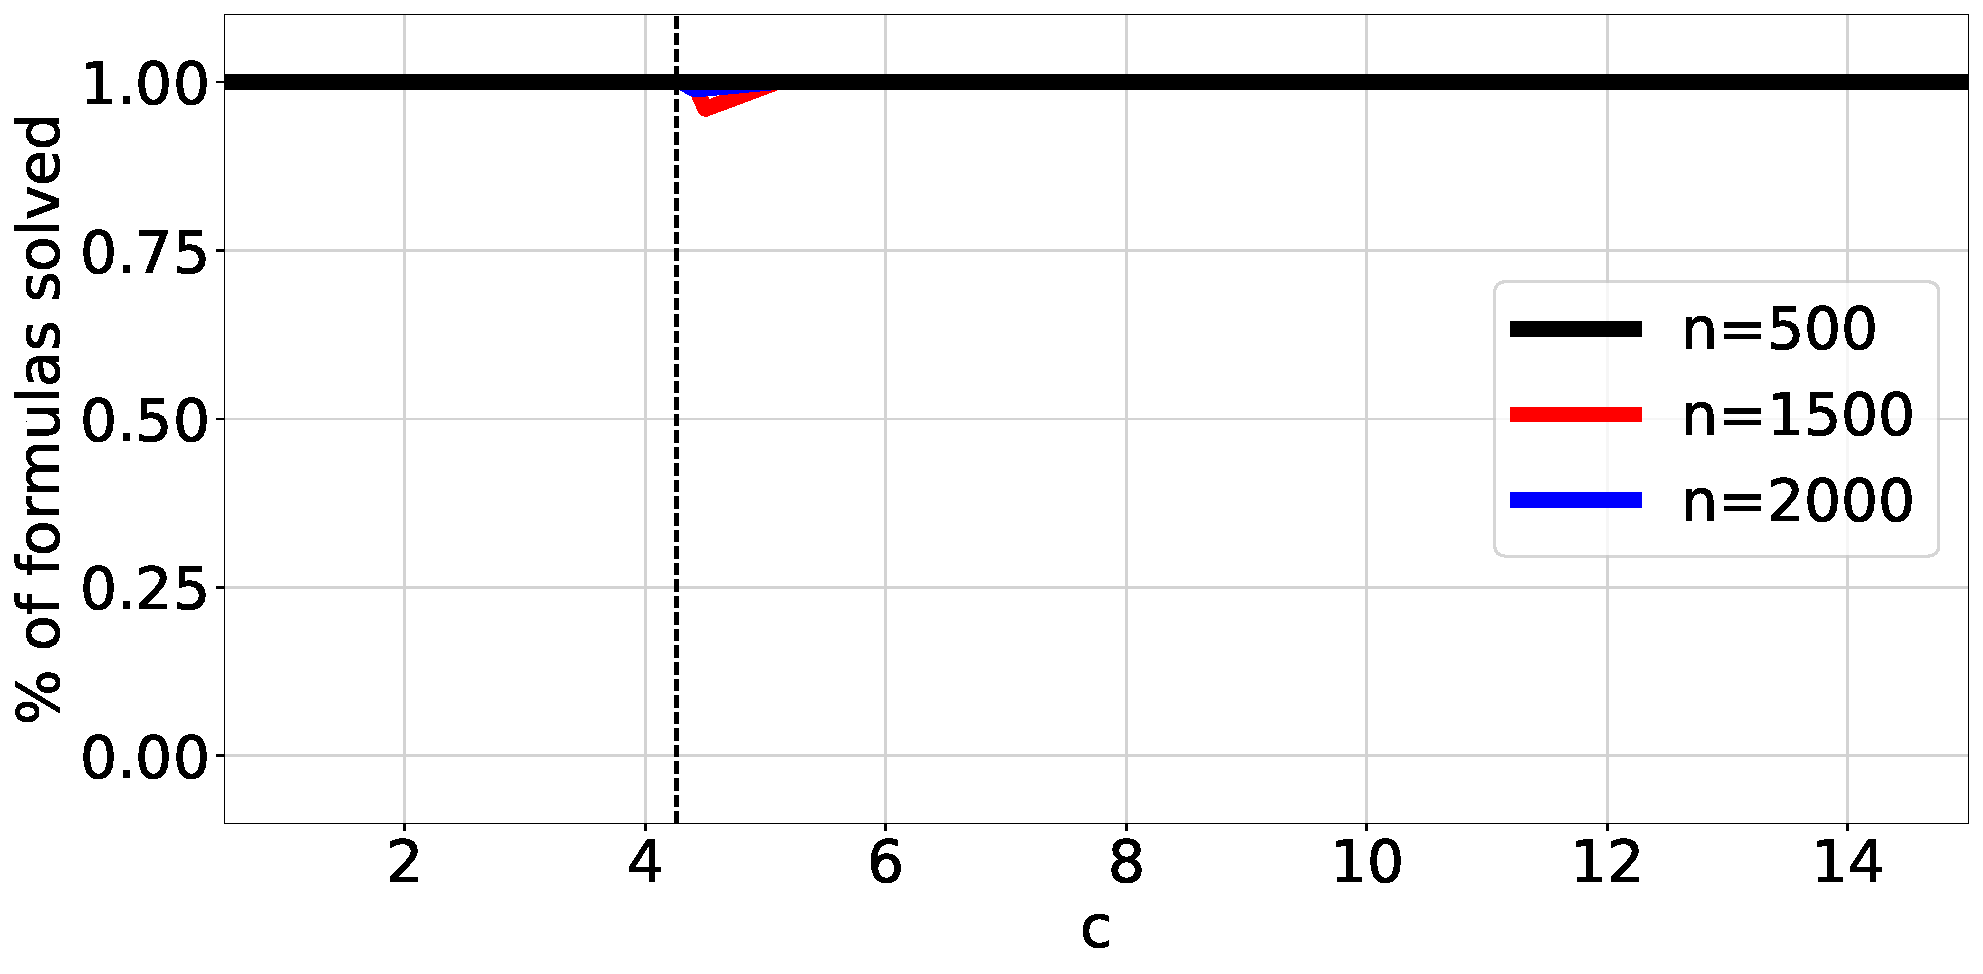
\includegraphics[
  width=\linewidth,
  height=4.35cm,
  keepaspectratio
]{assets/performance_planted sat assignment.pdf}

\vspace{0.25em}

{\scriptsize
Performance on planted SAT, averaged over 100 executions.
}
\end{center}

\column{0.49\textwidth}
\begin{center}
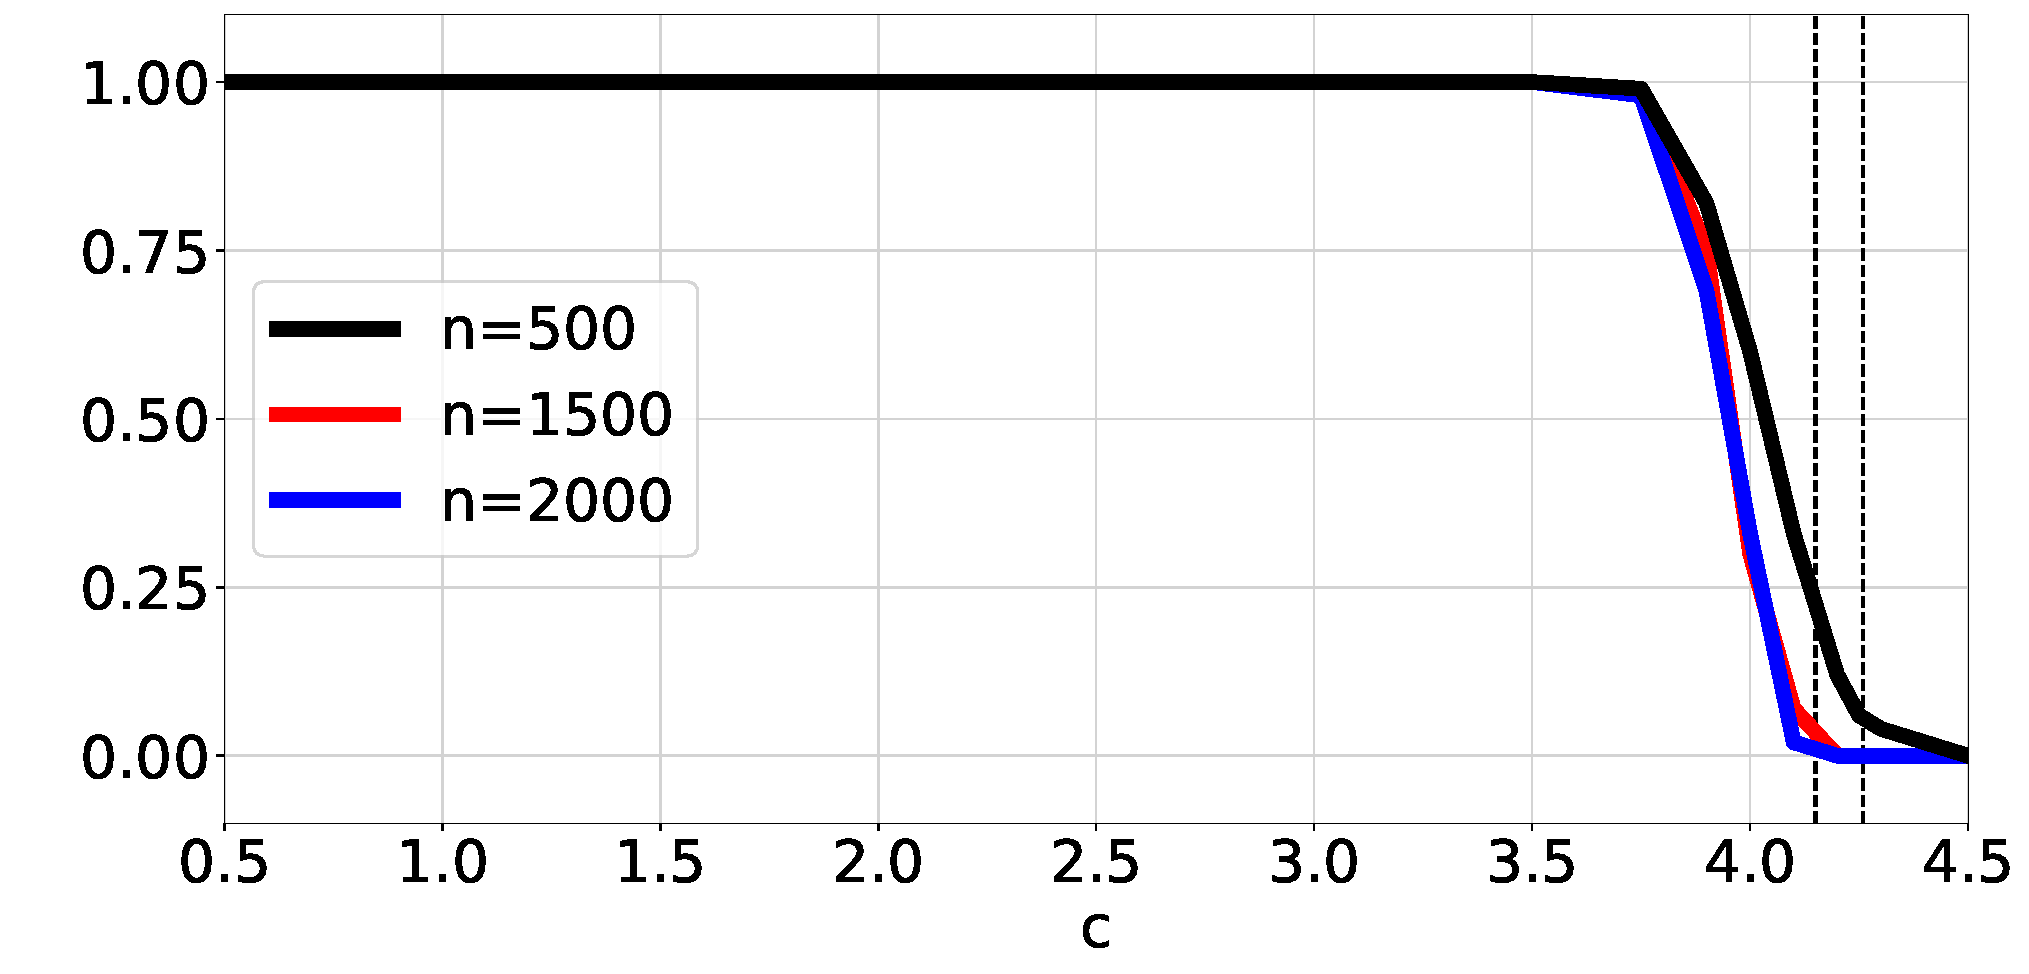
\includegraphics[
  width=\linewidth,
  height=4.35cm,
  keepaspectratio
]{assets/performance_random sat assignment.pdf}

\vspace{0.25em}
{\scriptsize
Random 3SAT; Vertical lines at \(c=4.15\) and \(c=4.26\);  
\(c \approx 3.9\) is the 1RSB phase transition, where curve starts dropping.  
}
\end{center}

\end{columns}

\vspace{0.45em}

\begin{center}
\begin{minipage}{0.94\textwidth}
\begin{block}{Insights}
\centering
\begin{itemize}
    \item No previous rigorous or empirical results for Planted SAT with $c$ just above the threshold
    \item Support not relevant for sparse formulas (``pure literals"--for another lecture)
\end{itemize}
\end{block}
\end{minipage}
\end{center}

\end{frame}


% ----------------------------------------------------------

% ------------------------------------------------------------
\begin{frame}{How support appears in the embeddings}

\small

\begin{columns}[T,onlytextwidth]

% ============================================================
% Left: two images
% ============================================================
\column{0.62\textwidth}

\begin{center}

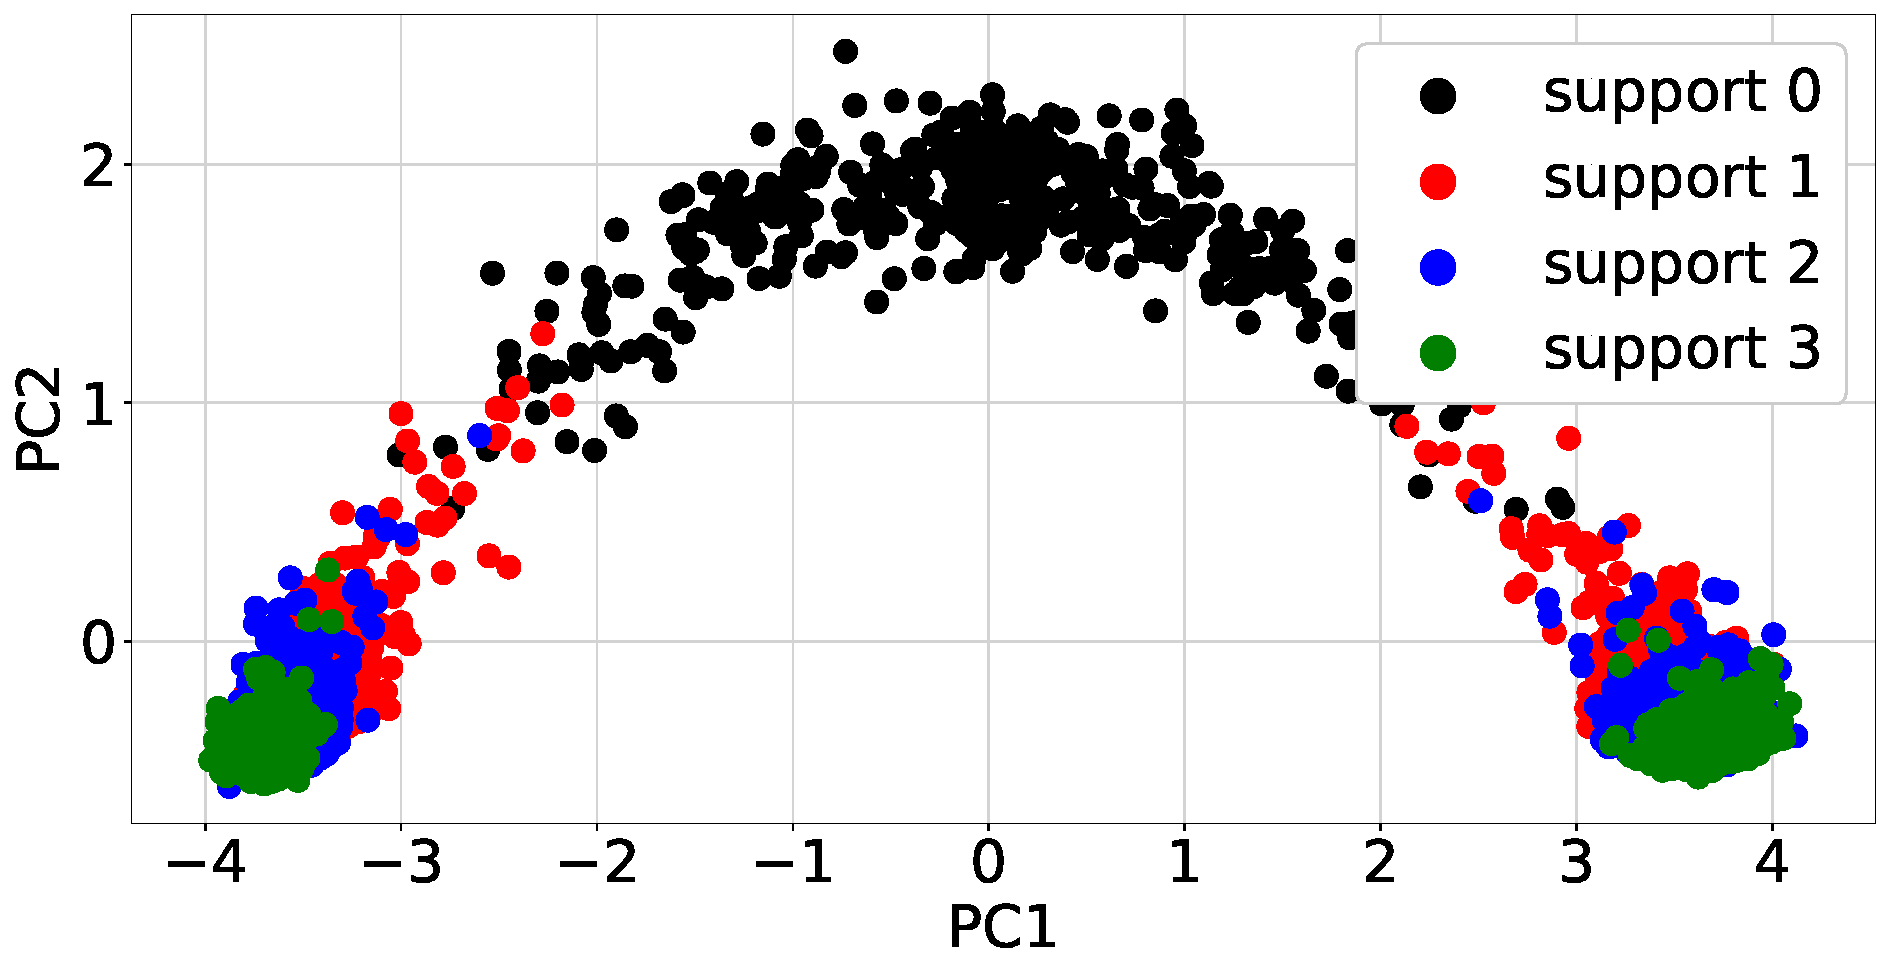
\includegraphics[
  width=0.88\linewidth,
  height=3.1cm,
  keepaspectratio
]{assets/good_support_color.pdf}

\vspace{0.35em}

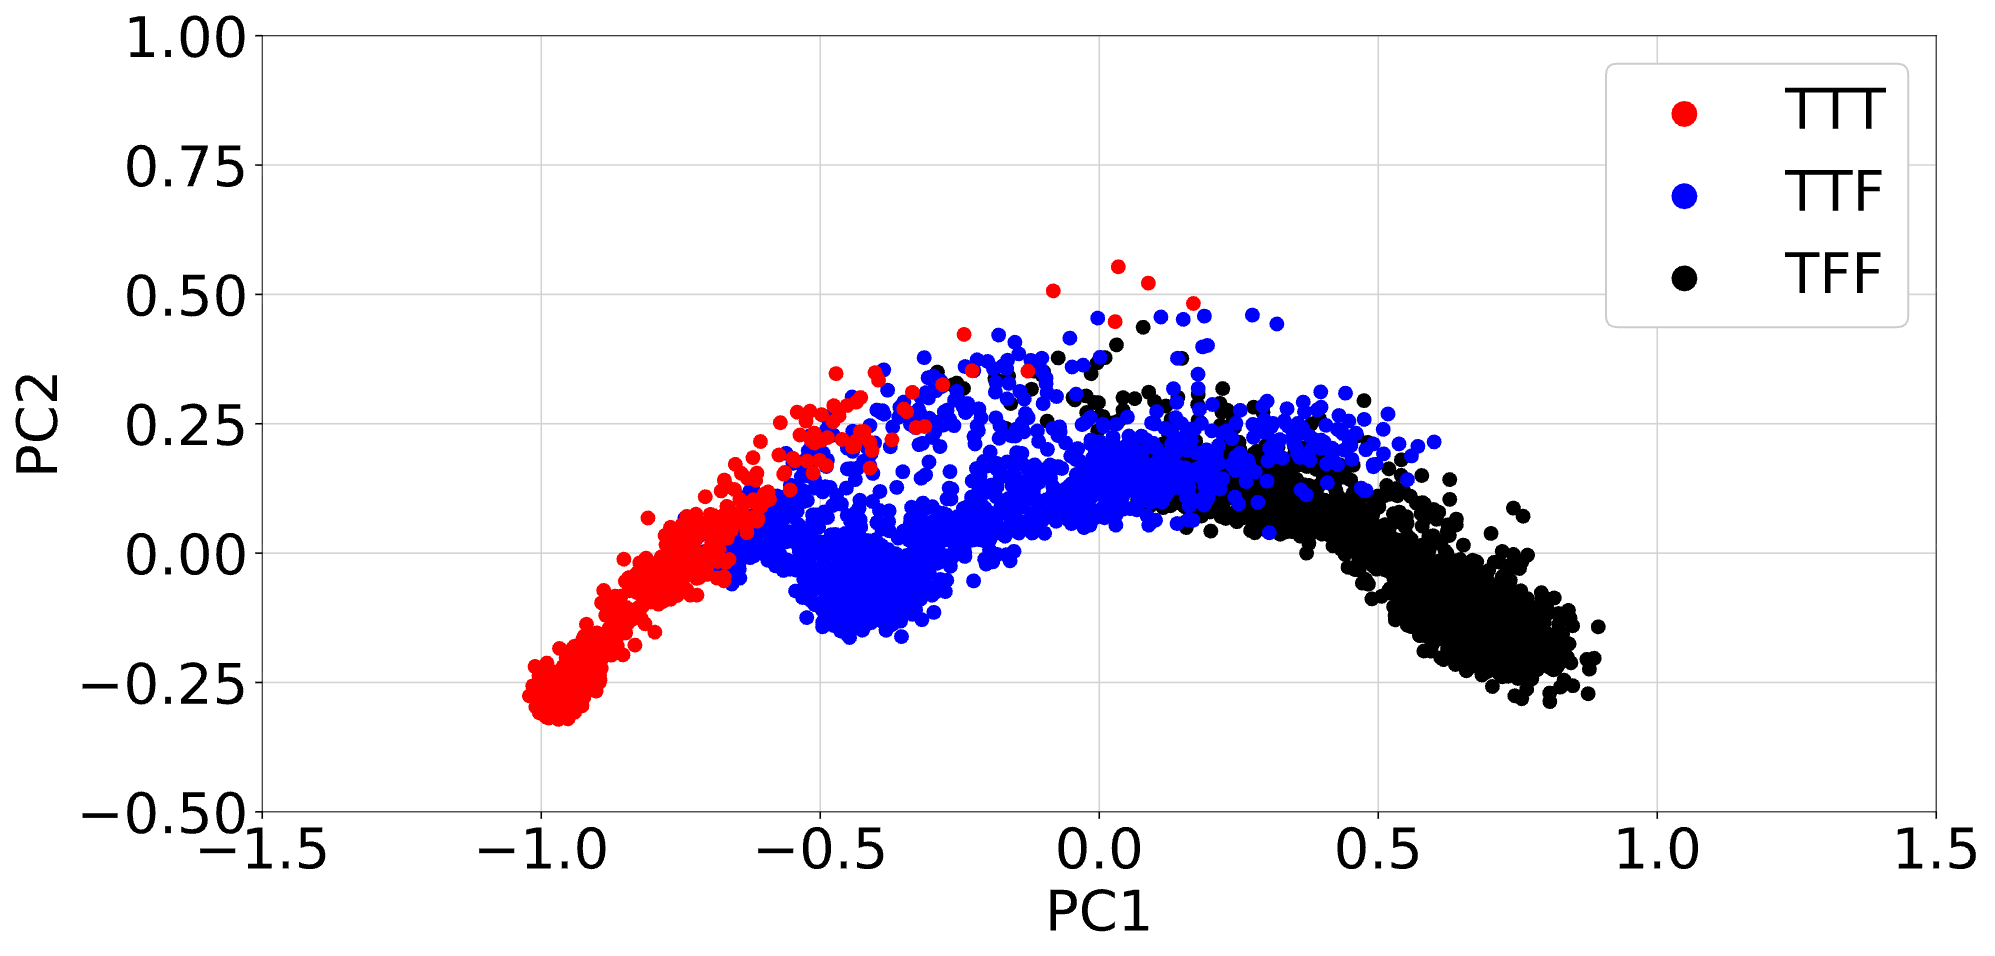
\includegraphics[
  width=0.88\linewidth,
  height=3.1cm,
  keepaspectratio
]{assets/clause_embedding.png}

\end{center}

% ============================================================
% Right: explanation / replacement figure
% ============================================================
\column{0.36\textwidth}

\begin{overlayarea}{\linewidth}{6.6cm}

\only<1-2>{
\vspace{4mm}

\textbf{Variable plane}
\[
\begin{aligned}
\mathrm{PC1}>0 &\quad \Longleftrightarrow \quad \text{literal is TRUE}\\
\mathrm{PC1}<0 &\quad \Longleftrightarrow \quad \text{literal is FALSE}
\end{aligned}
\]

\vspace{0.35em}

\textbf{Clause plane}
\[
\begin{aligned}
\mathrm{PC1}>0 &\quad \Longleftrightarrow \quad \text{TFF clause}\\
\mathrm{PC1}<0 &\quad \Longleftrightarrow \quad \text{other clause types}
\end{aligned}
\]

\only<2>{
\begin{center}
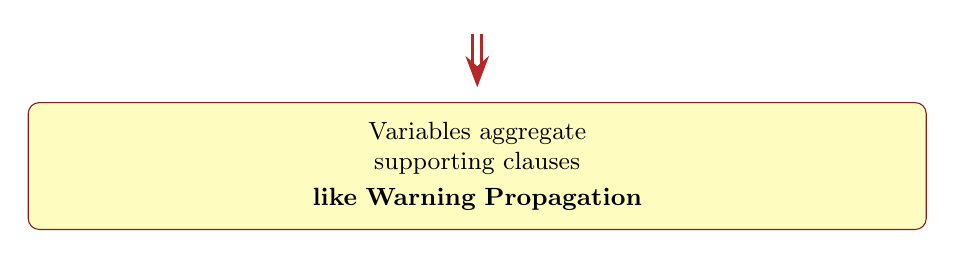
\begin{tikzpicture}[
    wpbox/.style={
        rounded corners,
        draw=emphcolor!75!black,
        fill=yellow!25,
        text width=0.90\linewidth,
        align=center,
        inner sep=7pt,
        font=\small
    }
]

\draw[
  ->,
  >=Stealth,
  double,
  double distance=2pt,
  line width=1.2pt,
  color=emphcolor
] (0,0.70) -- (0,0.02);

\node[wpbox] at (0,-0.98) {
Variables aggregate\\
supporting clauses\\[0.2em]
\textbf{like Warning Propagation}
};

\end{tikzpicture}
\end{center}
}
}

\only<3->{
\vspace{1mm}
\begin{center}
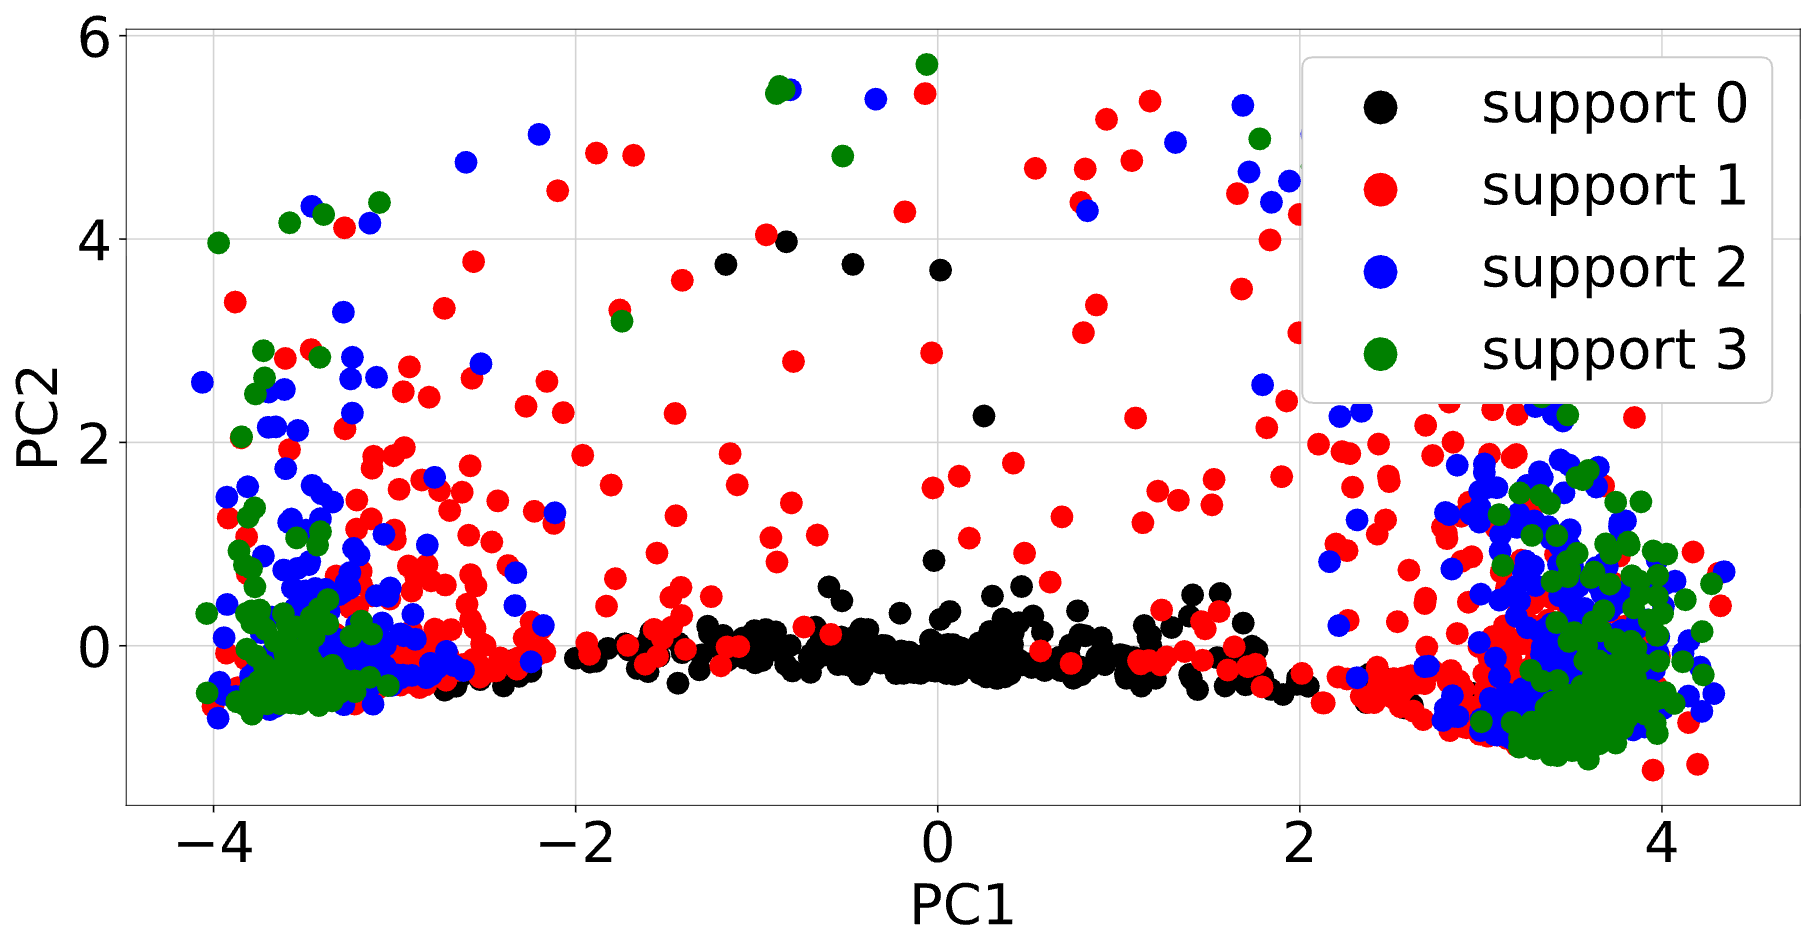
\includegraphics[
  width=\linewidth,
  height=5.2cm,
  keepaspectratio
]{assets/very_bad_support.png}
\end{center}
}

\end{overlayarea}

\end{columns}

\end{frame}
% ------------------------------------------------------------
\begin{frame}{From concept to a simpler GNN}

\small

\begin{block}{Idea}
Once we know the relevant concept is \textbf{support}, we can ask for the
simplest GNN that still learns it.
\end{block}

\vspace{0.5em}

We derived a simplified high-dimensional learned message-passing rule that performs like NeuroSAT:

\[
C^{t+1}
\longleftarrow
\tanh\!\left(FC_c\!\left(M^\top L^t\right)\right),
\]

\[
L^{t+1}
\longleftarrow
\tanh\!\left(
FC_l\!\left(M C^t\right)
+
FC_{\Delta}\!\left(L^t - \mathrm{Flip}(L^t)\right)
\right).
\]

\vspace{0.6em}

\begin{itemize}
    \item \(L^t\): literal embeddings at iteration \(t\)
    \item \(C^t\): clause embeddings at iteration \(t\)
    \item \(M\): literal--clause incidence matrix
    \item \(FC\): fully-connected layer, i.e. matrix multiplication plus bias
    \item \(\mathrm{Flip}(L^t)\): swaps each literal embedding with its negation
\end{itemize}

\vspace{0.4em}

\begin{center}
\textcolor{blue!70!black}{
\textbf{A learned message-passing algorithm, almost linear, and can be analyzed.}
}
\end{center}

\end{frame}
% ----------------------------------------------------------
% ------------------------------------------------------------
\begin{frame}{A simplified GNN can be analyzed}

\small

\only<2->{
\begin{tikzpicture}[remember picture,overlay]
\node[anchor=north east, xshift=-0.35cm, yshift=-3.3cm] at (current page.north east) {
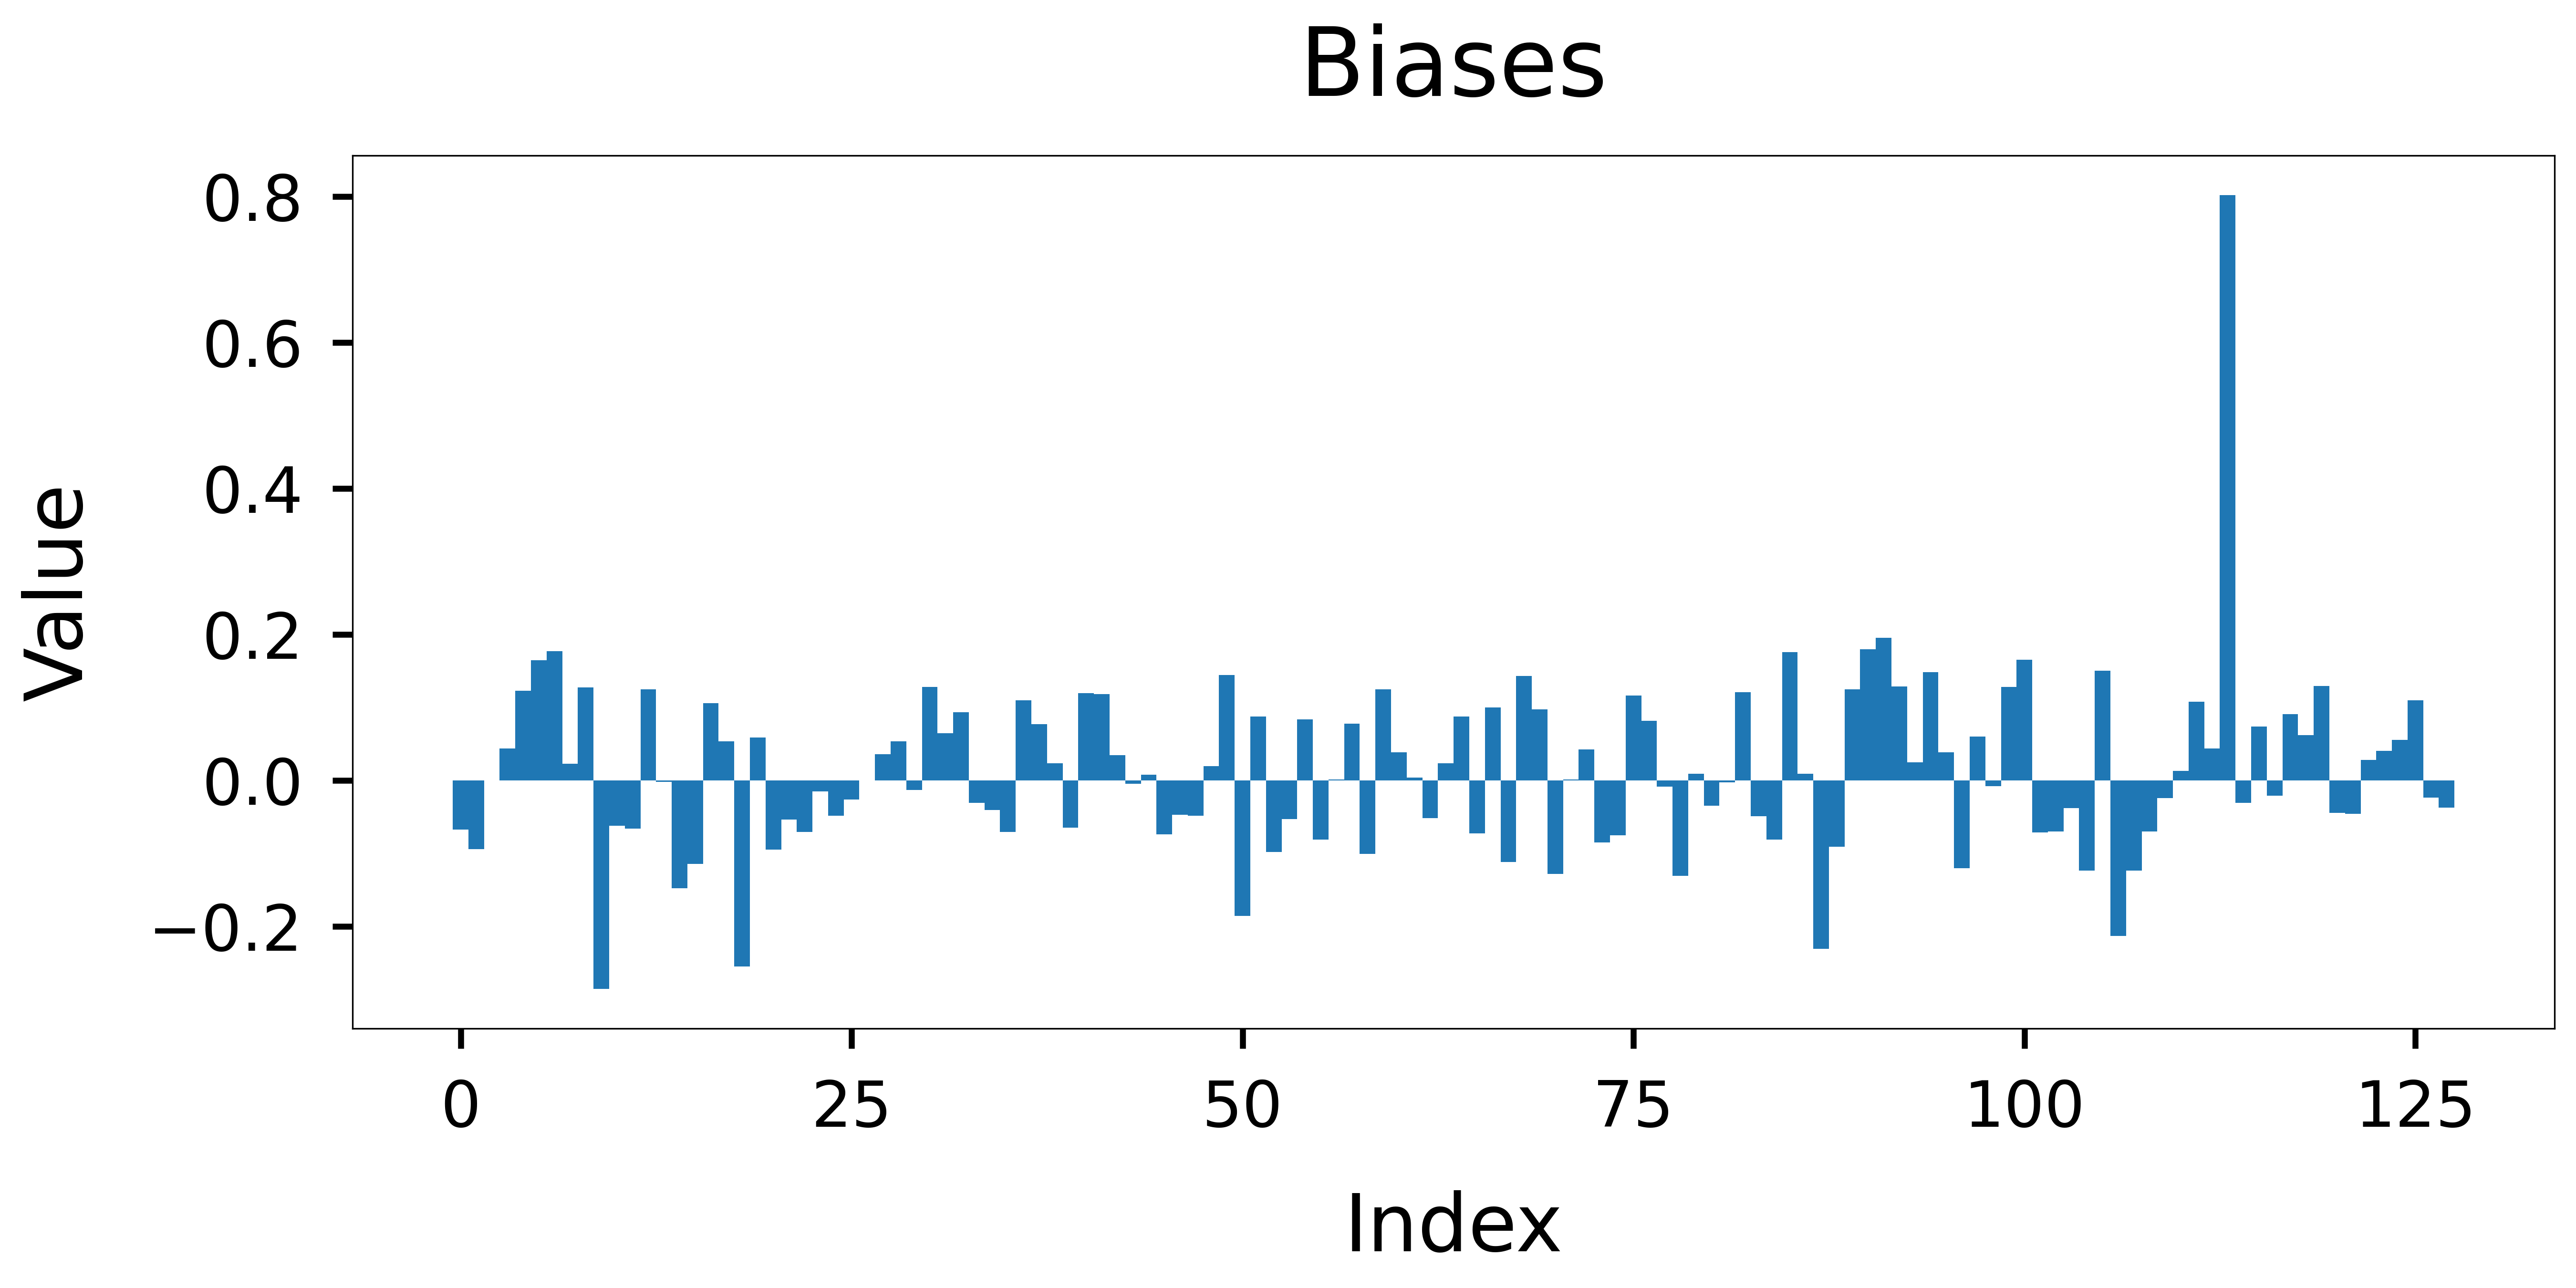
\includegraphics[
  width=0.38\textwidth,
  height=3.0cm,
  keepaspectratio
]{assets/bias_plots.png}
};
\end{tikzpicture}
}

\textbf{Assume:}
\begin{itemize}
    \item \(d=1\), and \(L^0=\mathbf{1}_{2n}\).
    \item The input is a Planted \(3\)-CNF formula with \(m=cn\) clauses, $c$ sufficiently larger constant.
\item The parameters satisfy the required sign pattern:
\[
\hspace*{-14em}
a_l,b_l,a_{\Delta},b_{\Delta},b_c>0,\quad a_c<0,
\]
\alt<2->{\textcolor{red!75!black}{\textbf{with \(b_c\) sufficiently large.}}}{with \(b_c\) sufficiently large.}
\end{itemize}

\vspace{0.4em}

\textbf{Then:}
With high probability, for every \(t\ge 2\),

\[
0.75
\le
c_{\texttt{TTT}}^t
<
c_{\texttt{TTF}}^t
<
c_{\texttt{TFF}}^t .
\]

Moreover, for every \(t\ge 1\), every positive literal \(l_i\) under the planted, and every negative literal \(l_j\),

\[
0.75 < l_j^t < l_i^t .
\]

\vspace{0.5em}


\end{frame}

% ------------------------------------------------------------
\begin{frame}{From GNN to WalkSAT}

\begin{columns}[T,onlytextwidth]

\column{0.49\textwidth}
\begin{center}
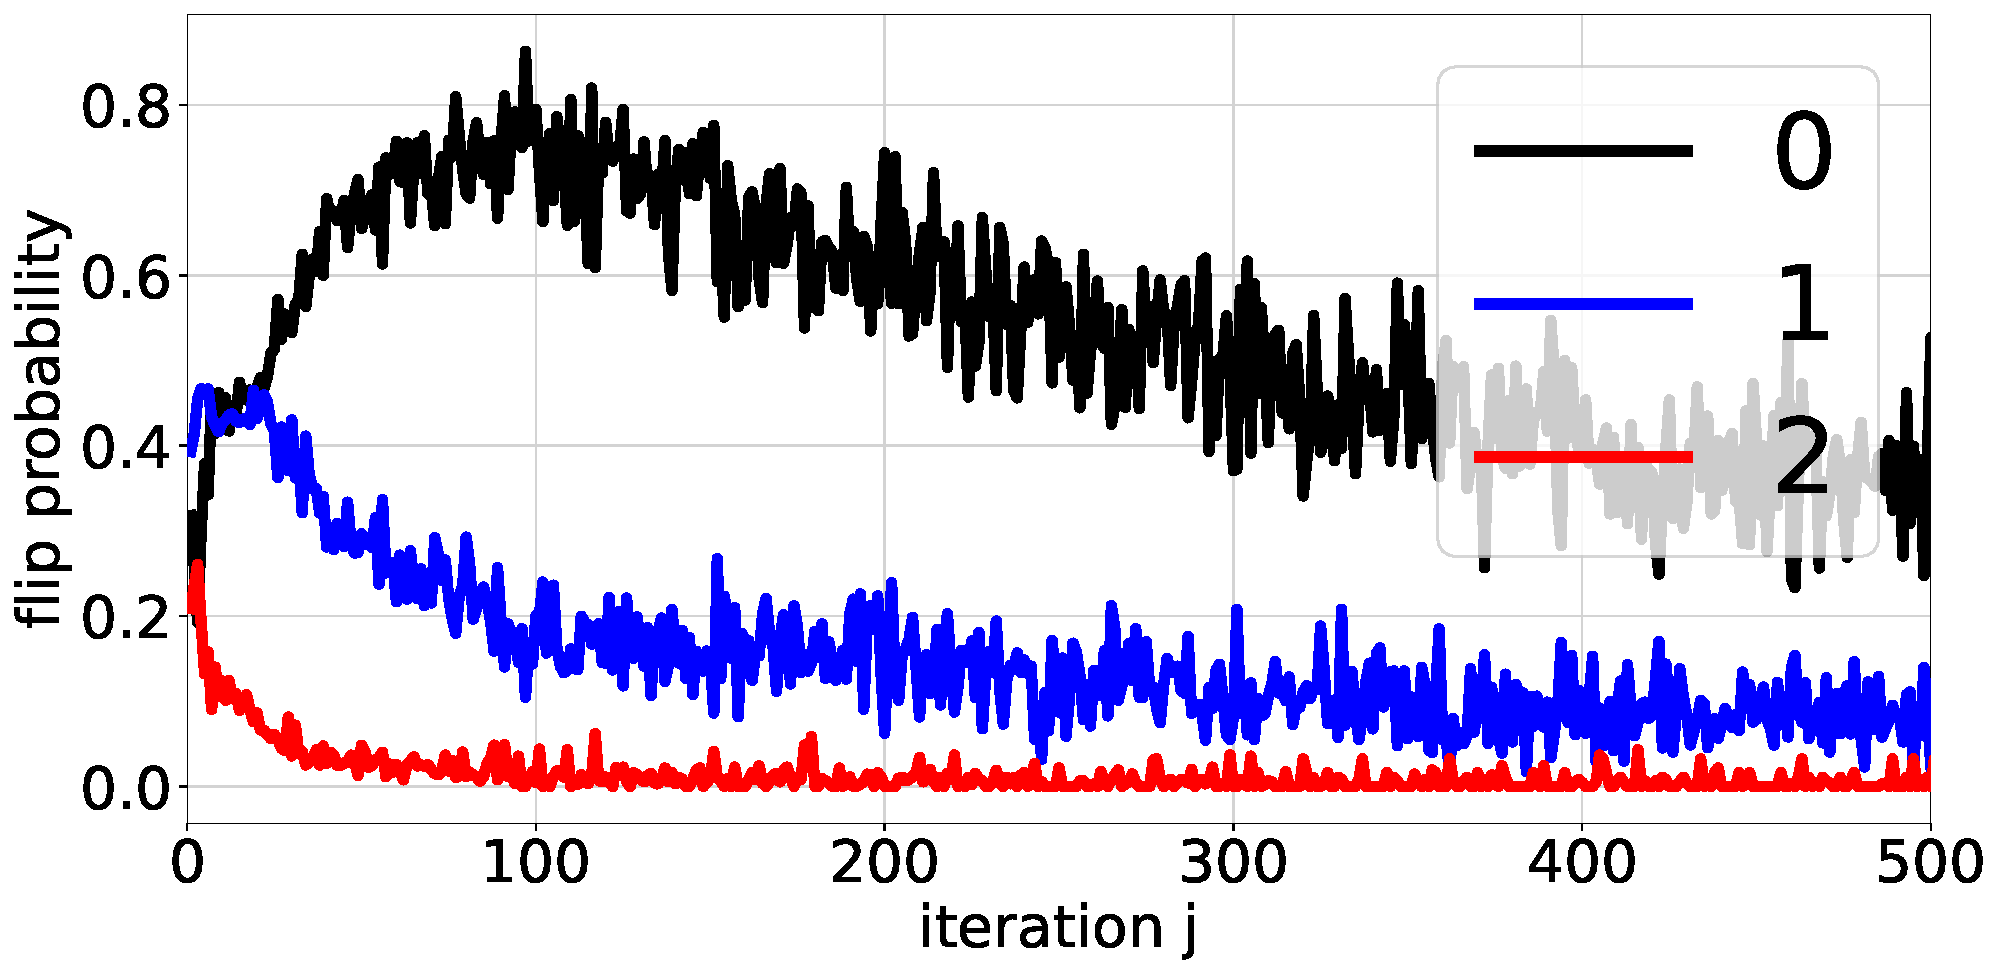
\includegraphics[
  width=\linewidth,
  height=4.2cm,
  keepaspectratio
]{assets/matplot_support_iter1.pdf}

\vspace{0.25em}

{\scriptsize
Flip probability is inversely proportional to support.
}
\end{center}

\column{0.49\textwidth}
\begin{center}
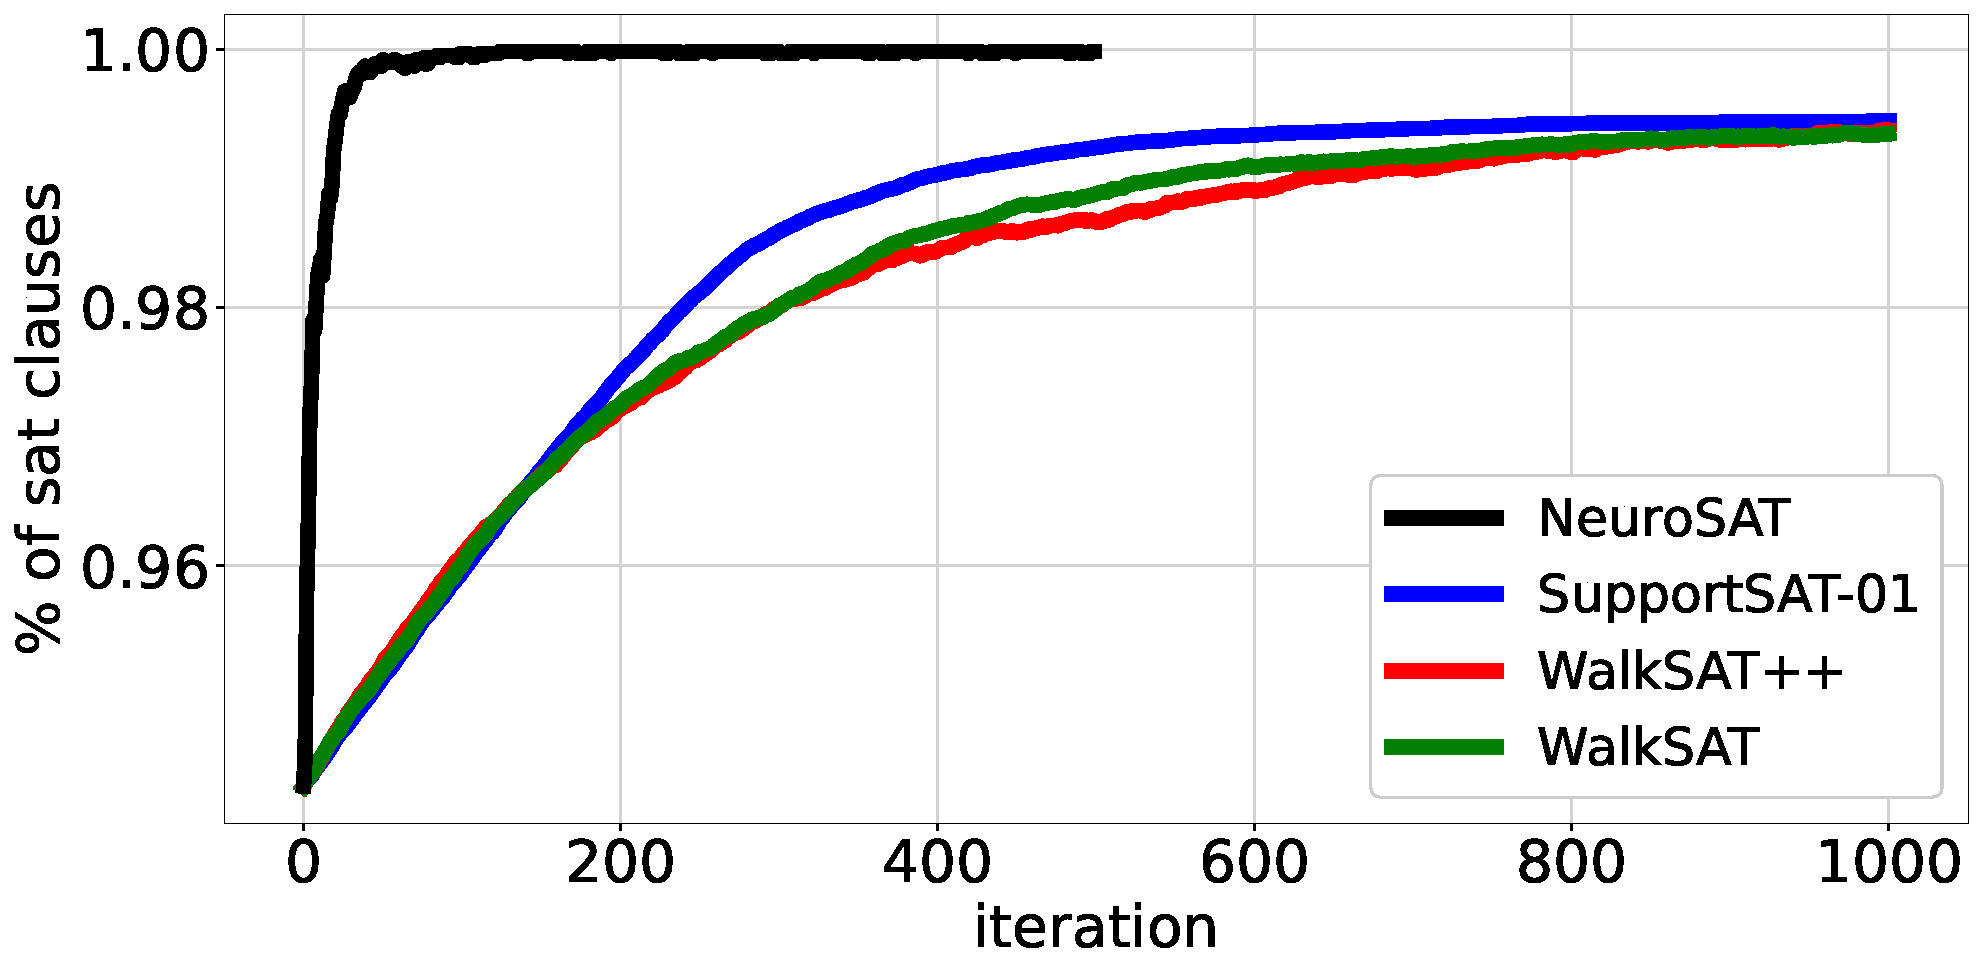
\includegraphics[
  width=\linewidth,
  height=4.2cm,
  keepaspectratio
]{assets/walksat2.pdf}

\vspace{0.25em}

{\scriptsize
The support-inspired heuristic improves WalkSAT.
}
\end{center}

\end{columns}

\vspace{0.55em}

\onslide<2->{
\begin{center}
\begin{minipage}{0.78\textwidth}
\begin{block}{Toy Insight}
\centering
The concept learned by the GNN can be translated back into a hand-crafted local-search heuristic.
\end{block}
\end{minipage}
\end{center}
}

\end{frame}

\begin{frame}{Graph coloring: the simplex geometry}

\begin{columns}[T,onlytextwidth]

% ============================================================
% Left: two PCA images
% ============================================================
\column{0.50\textwidth}

\begin{center}
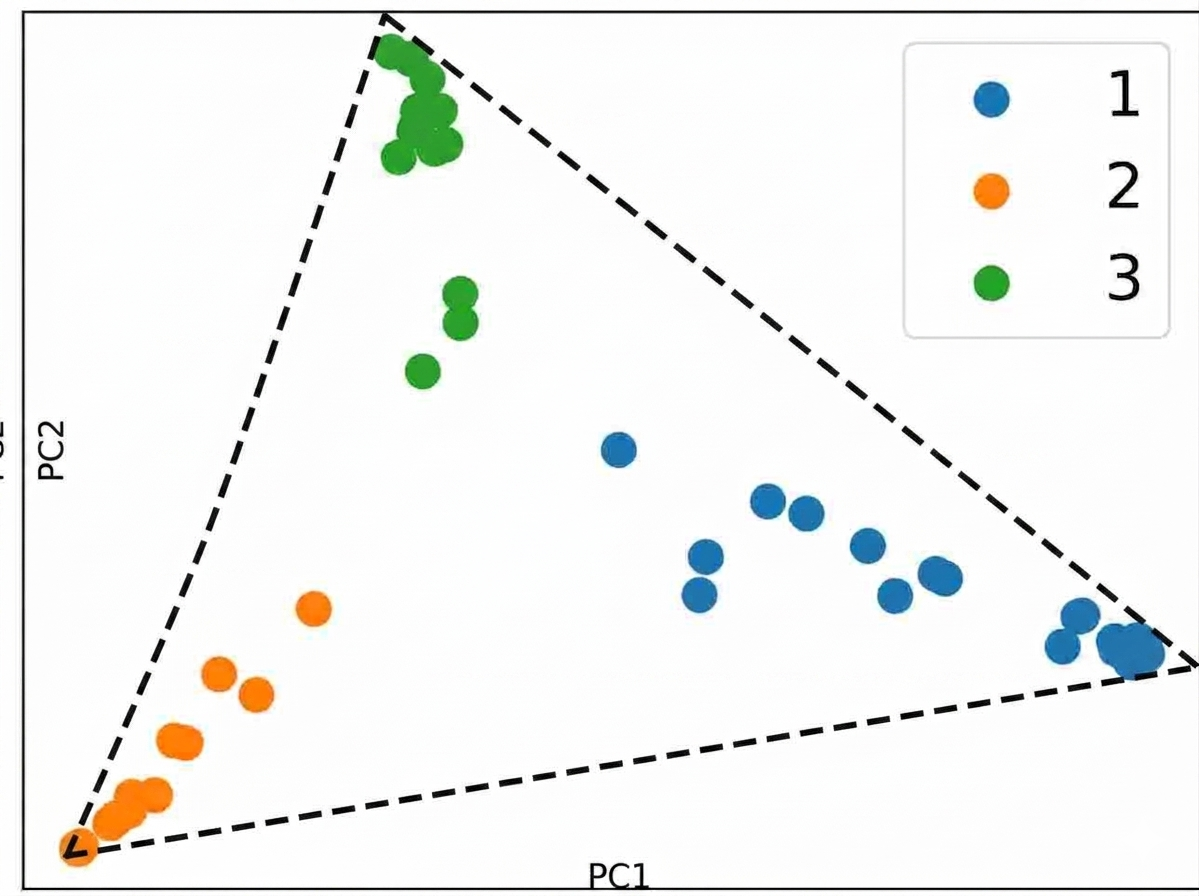
\includegraphics[
  width=0.92\linewidth,
  height=3.0cm,
  keepaspectratio
]{assets/good_scatter_coloring.png}

\vspace{0.05em}

{\scriptsize Good coloring: embeddings organize into a simplex}

\vspace{0.35em}

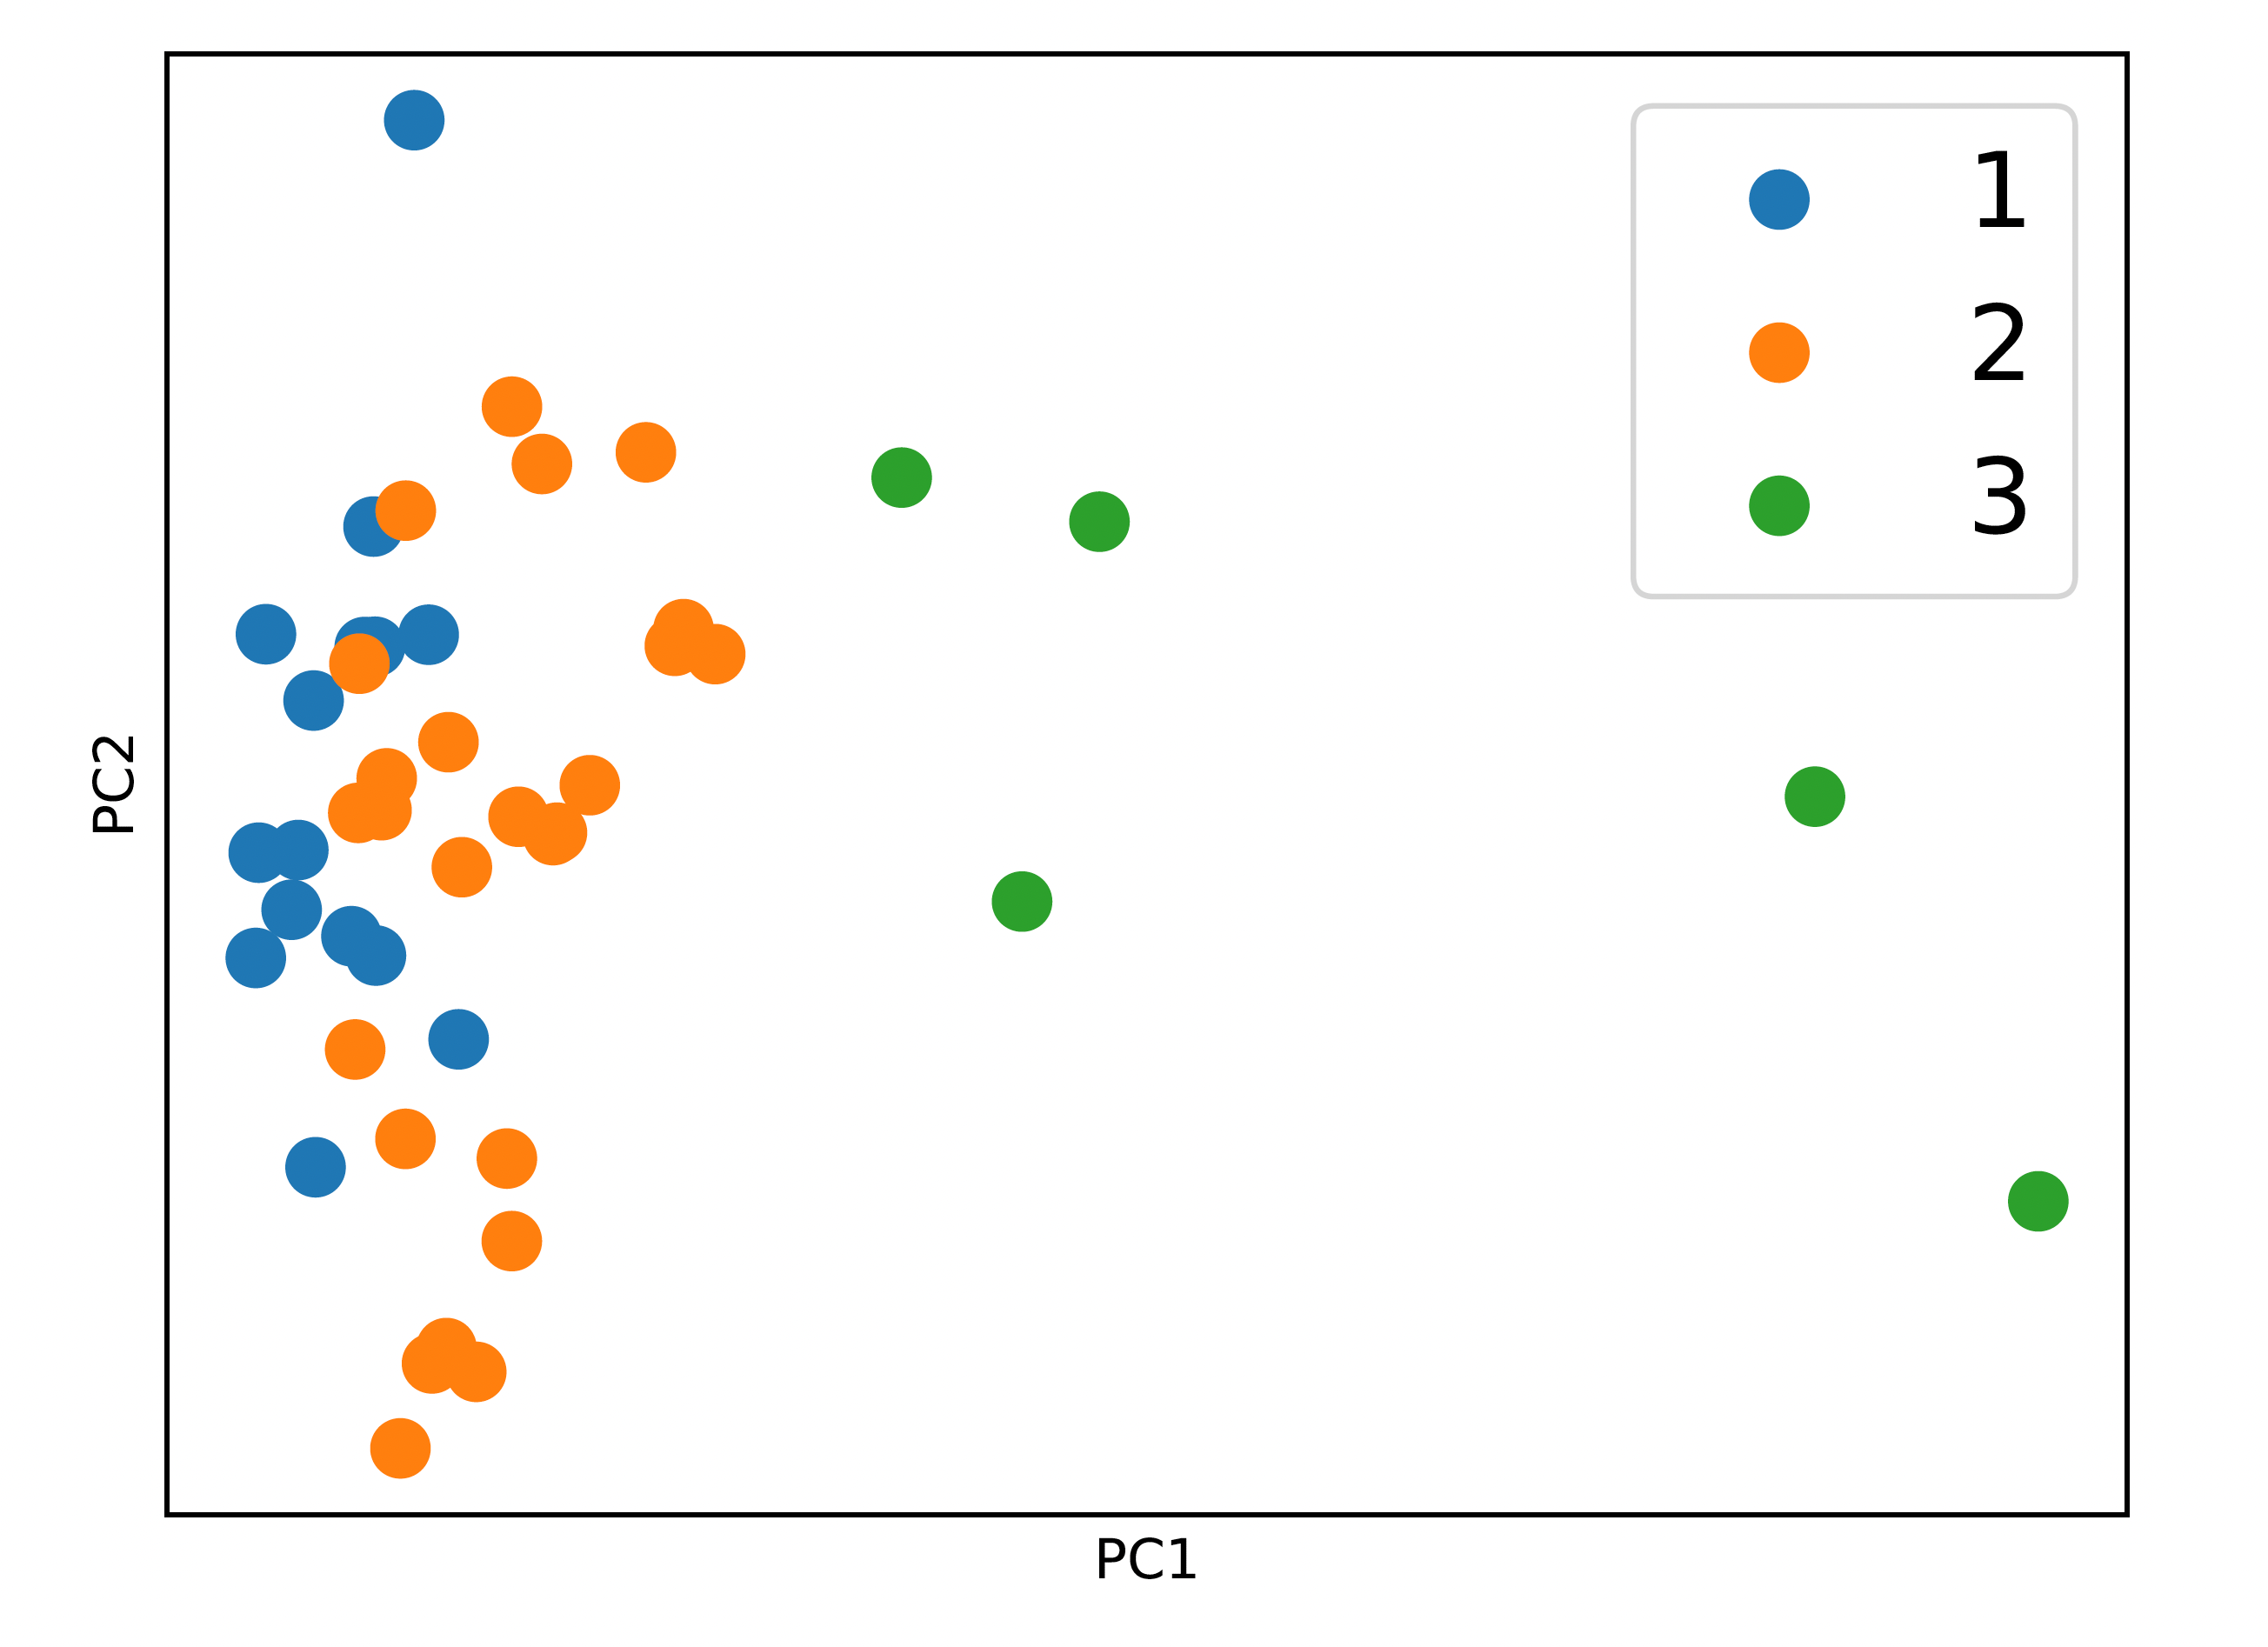
\includegraphics[
  width=0.92\linewidth,
  height=3.0cm,
  keepaspectratio
]{assets/bad_3col_embedding.png}

{\scriptsize Bad coloring: the simplex structure is weak or missing}
\end{center}

% ============================================================
% Right: explanation
% ============================================================
\column{0.47\textwidth}

\textbf{GNN-\GCP} (Lemos et al., 2019):
\begin{itemize}\small
  \item Trained for \(3\)-colorability
  \item Message-passing LSTM with \(64\)-dimensional 
  \item Fails on 95\% of the instances
embeddings
\end{itemize}

\medskip

\textbf{Support in coloring:}
\[
\operatorname{supp}_{\sigma}(v)
=
\min_{c \neq \sigma(v)}
\left|
\{u\in N(v):\sigma(u)=c\}
\right|.
\]

\medskip

\textbf{2D PCA projection:}
\begin{itemize}\small
  \item Embeddings form a \textbf{triangle}
  \item Color classes cluster near the \textbf{corners}
  \item High-support vertices move toward corners
  \item Low-support vertices stay closer to the center
\end{itemize}



\end{columns}


\end{frame}

% ----------------------------------------------------------
% ------------------------------------------------------------
\begin{frame}{\OptGNN~(Yau et al., NeurIPS 2024)}

\begin{columns}[c,onlytextwidth]

% ---------------- left: image ----------------
\column{0.62\textwidth}

\begin{center}
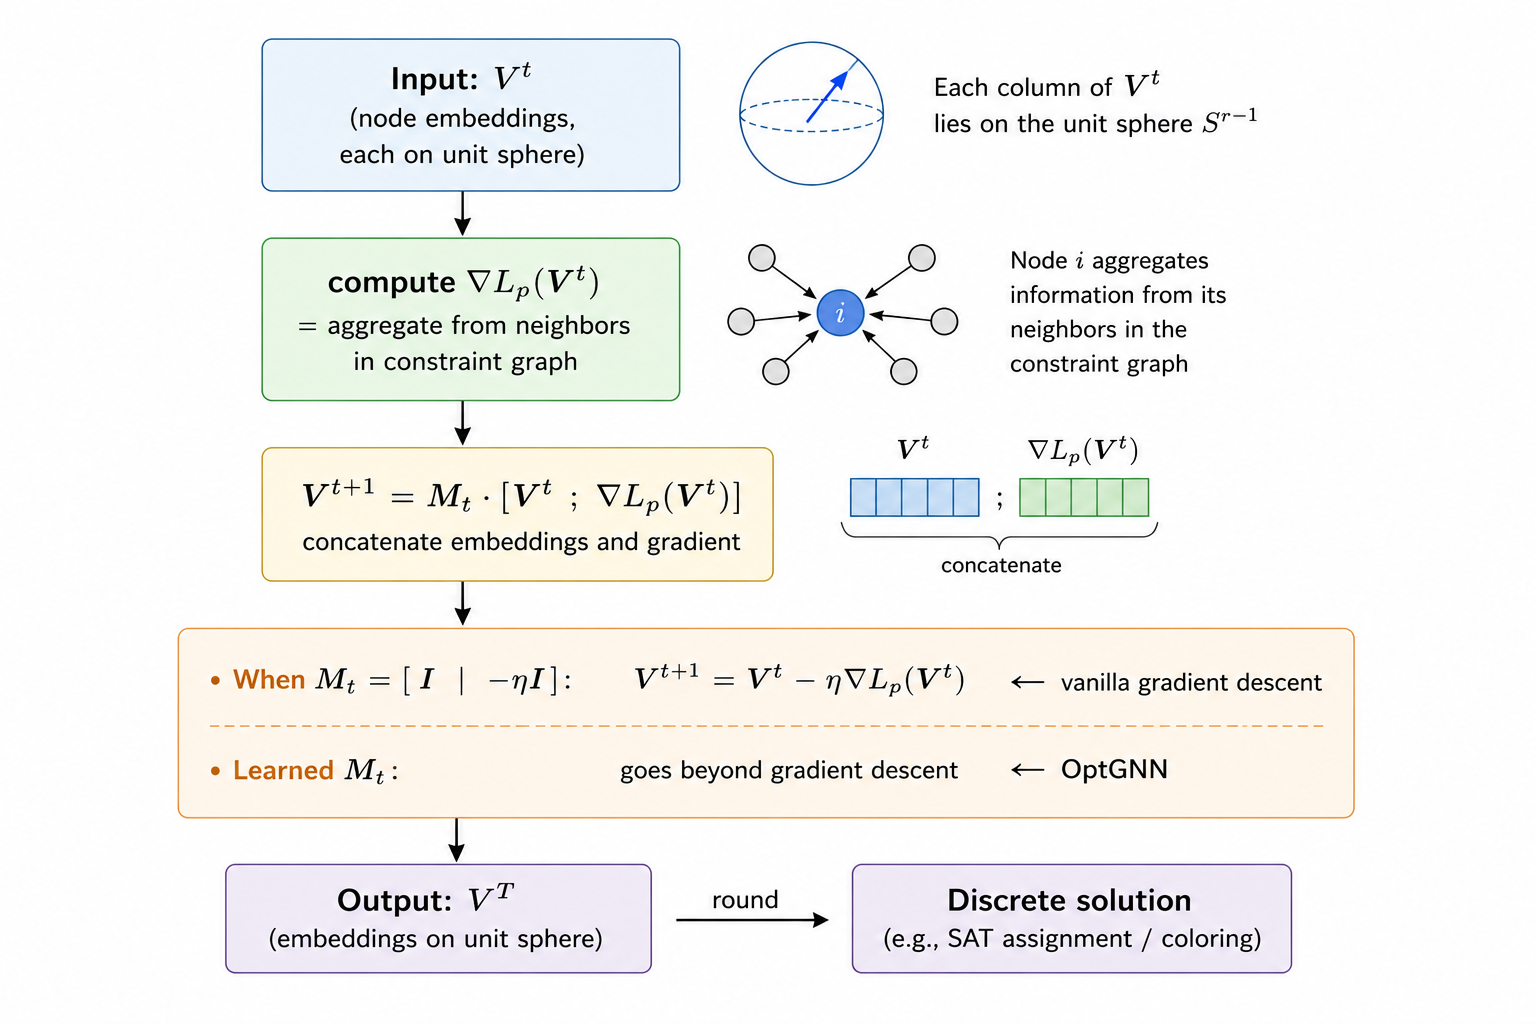
\includegraphics[
  width=\linewidth,
  height=0.78\textheight,
  keepaspectratio
]{assets/OptGNN.png}
\end{center}

% ---------------- right: explanation ----------------
\column{0.35\textwidth}

\small

\begin{itemize}
    \item \(L_{\rho}\) is the penalized SDP Lagrangian.

    \vspace{0.6em}

    \item \(\nabla L_{\rho}(V^t)\) is the message-passing component:
    nodes aggregate information through the constraint graph.

    \vspace{0.6em}

    \onslide<2->{

    \item It is a general optimization GNN built by learning around an SDP-style update.

    \vspace{0.6em}

    \item \textcolor{red!75!black}{On SAT, OptGNN reaches \(98\%\)--\(99\%\) approximation,
never learns support, never solves.}
 
    }
\end{itemize}

\end{columns}

\end{frame}

% ------------------------------------------------------------
\begin{frame}{\OptGNN + our augmentation}

\begin{columns}[c,onlytextwidth]

% ---------------- left: image ----------------
\column{0.70\textwidth}

\begin{center}
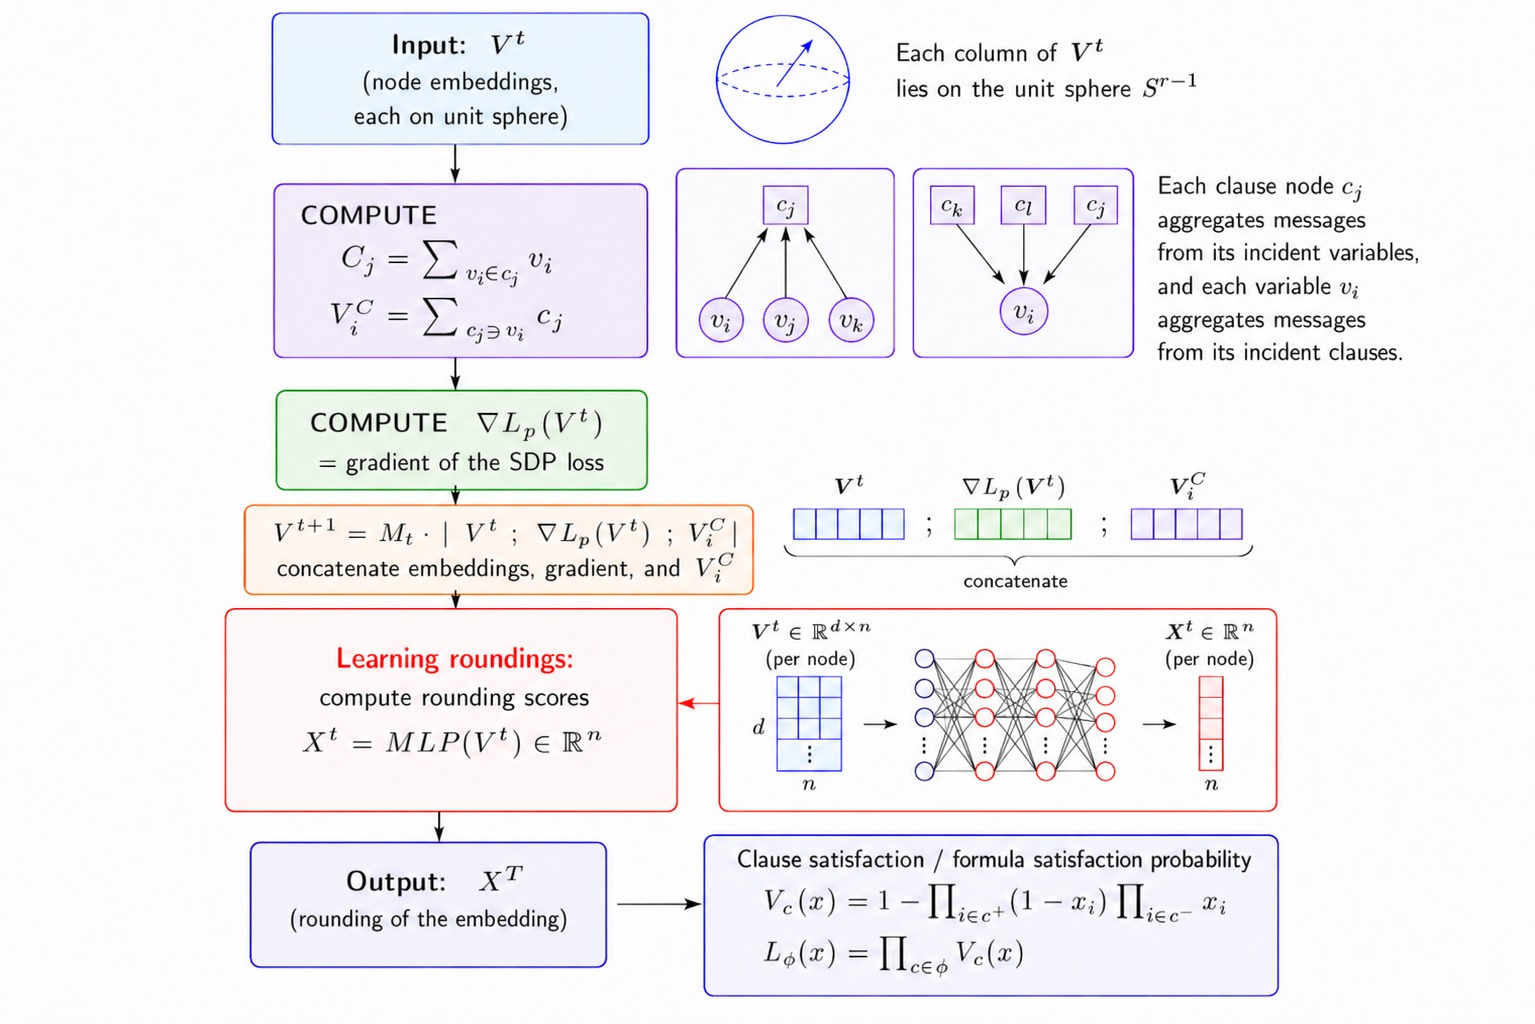
\includegraphics[
  width=1.06\linewidth,
  height=0.86\textheight,
  keepaspectratio
]{assets/Augmented-OptGNN.jpeg}
\end{center}

% ---------------- right: explanation ----------------
\column{0.28\textwidth}

\small

\textbf{Original OptGNN:}
\begin{itemize}
    \item SDP-inspired optimizer
    \item \(98\%\)--\(99\%\) approximation
    \item no support, no exact solving
\end{itemize}

\vspace{0.5em}

\onslide<2->{
\textbf{We add:}
\begin{itemize}
    \item clause aggregation
    \item SAT Objective loss
\end{itemize}
}

\vspace{0.5em}

\onslide<3->{
\textbf{Result:}
\begin{itemize}
    \item SAT Objective loss: solves up to \(c\approx 3.0\)
    \item + clause aggregation: solves up to \(c\approx 3.9\)
\end{itemize}
}

\end{columns}

\end{frame}
% ------------------------------------------------------------
\begin{frame}{Open problems}

\small
\renewcommand{\arraystretch}{1.35}

\begin{tabular}{@{}p{0.28\textwidth}p{0.66\textwidth}@{}}
\toprule
\rowcolor{gray!15}
\textbf{Problem} & \textbf{Question} \\
\midrule

\uncover<1->{\textbf{\NeuroSAT~beyond \(d=1\)}}
&
\uncover<1->{Prove support tracking for \(d>1\) and for non-planted random 3-SAT.}
\\

\midrule

\uncover<2->{\textbf{High-Dimensional MP}}
&
\uncover<2->{\NeuroSAT's messages are basically one-dimensional (PC1). Can we take real advantage of a HD setting?}
\\

\midrule

\uncover<3->{\textbf{Symmetry breaking in \GCP}}
&
\uncover<3->{Coloring is permutation symmetric. Help the GNN break symmetry. Spectral features?}
\\

\midrule

\uncover<4->{\textbf{Can GNNs learn something genuinely new?}}
&
\uncover<4->{\OptGNN~gives 99\% approximation, but does not learn support. What does it learn instead?}
\\

\midrule

\uncover<5->{\textbf{Architecture threshold}}
&
\uncover<5->{Is there a sharp transition in architecture space separating models that approximate from models that solve?}
\\

\midrule

\uncover<6->{\textbf{Are GNNs really worth it?}}
&
\uncover<6->{Show a problem and/or GNN architecture that beats all known hand-crafted heuristics.}
\\

\bottomrule
\end{tabular}

\end{frame}
% ----------------------------------------------------------

% ------------------------------------------------------------
\begin{frame}[plain]

\begin{center}
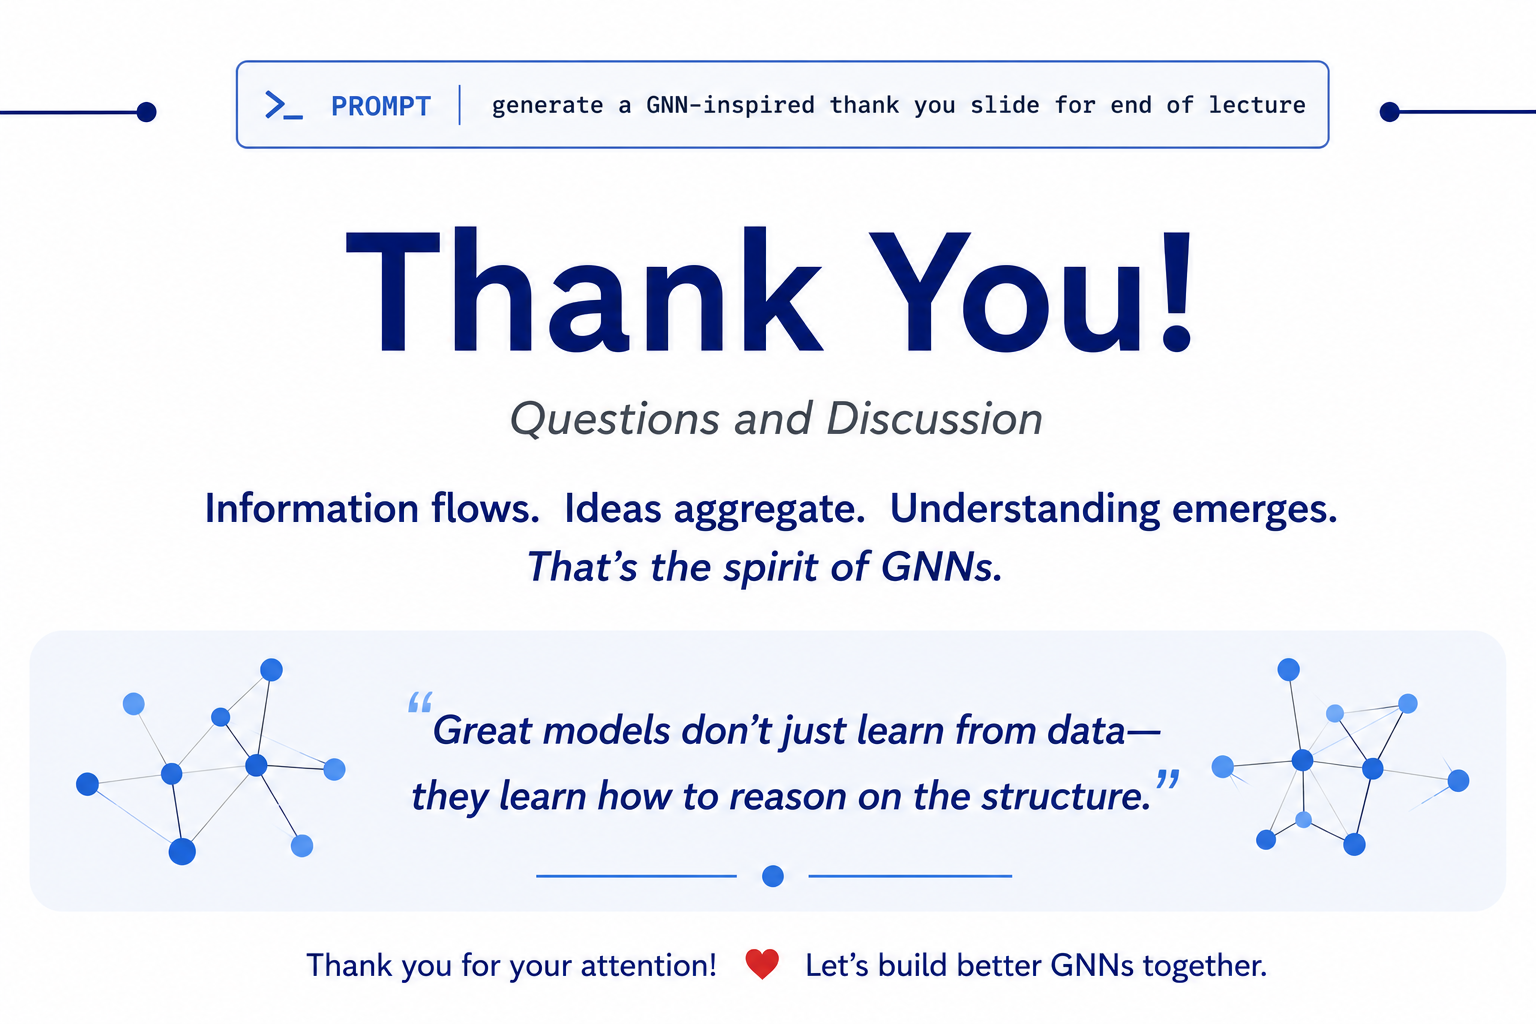
\includegraphics[
  width=\paperwidth,
  height=\paperheight,
  keepaspectratio
]{assets/thank_you.png}
\end{center}

\end{frame}

\end{document}

